\documentclass[]{article}
\usepackage{amsmath}
\usepackage{graphicx}
\usepackage{caption,subfigure} %float=figuras flotantes.
\usepackage{cases}
\usepackage{color} %red, green, blue, yellow, cyan, magenta, black, white
%\usepackage[table,xcdraw]{xcolor}
\usepackage[usenames,dvipsnames,svgnames,table,x11names,xcdraw]{xcolor} 
\usepackage{multirow}
\usepackage{tabularx}
\usepackage{hhline}
\usepackage{floatrow}
\definecolor{mygreen}{RGB}{28,172,0} % color values Red, Green, Blue
\definecolor{mylilas}{RGB}{170,55,241}
\setlength{\arrayrulewidth}{1mm}
\setlength{\tabcolsep}{18pt}
%\renewcommand{\arraystretch}{2.5}
\setlength{\textwidth}{170mm}\setlength{\textheight}{230mm}
\setlength{\oddsidemargin}{1mm}\setlength{\evensidemargin}{1mm}
\setlength{\topmargin}{-20mm}
\setlength{\parindent}{0mm} 

%---- Salto de línea en parrafo --------------------------------------------
\usepackage{parskip}
\setlength{\parindent}{0pt}	

%---- Hyperlinks ----------------------------------------------------------
\usepackage[ %
breaklinks , %
colorlinks =true , %
linkcolor =blue , %
citecolor =blue , %
urlcolor = blue %
]{ hyperref }


%---- Usar otros fonts + símbolo \degree -----------------------------------
\newcommand*{\myfont}{\fontfamily{lmtt}\selectfont}
\DeclareTextFontCommand{\textmyfont}{\myfont}	
\usepackage{gensymb} 

%---- Code highlighting con Listings ---------------------------------------
\usepackage{listings}	
\definecolor{mygreen}{rgb}{0.5,0.6,0.5}
\definecolor{mygray}{rgb}{0.5,0.5,0.5}
\definecolor{mymauve}{rgb}{0.58,0,0.82}
\definecolor{mygray2}{rgb}{0.9764, 0.9764, 0.9762}
%---- Config listings ------------------------------------------------------
\lstset{ %
	backgroundcolor=\color{mygray2},	% background color
	basicstyle=\footnotesize\ttfamily,	% tamaño de las letras y tipo de letra
	breaklines=true,	% corte de linea (line breaking)solo en espacio blanco
	captionpos=b,		% posicion del caption b,t,n (top,bottom,none)
	commentstyle=\color{ForestGreen},	% estilo del comentario
	%escapeinside={\%*}{*},	% si se desea agregar codigo Latex dentro el codigo debe ser %*codigo latex*
	frame=none,	% agrega marco al codigo
	frameround=tttt,	% redondear el marco
	keepspaces=true,	% mantiene los espacios en el texto, util para mantener la indentacion del codigo (uso posible en columns=flexible)
	keywordstyle=\color{blue},	% estilo de los keywords
	stringstyle=\color{mymauve},	% estilo del string
	numbers=none,	% donde poner los numeros de linea, (none, left, right)
	numbersep=5pt,	% cuan lejos los numeros de linea estan del codigo
	xleftmargin=0pt,	% margen izquierdo
	showspaces=false,	% muestra espacios de codigo en todas partes usando el caracter barra baja "_", sobreescribe el comando 'showstringspaces'
	showstringspaces=false,	% muestra espacios solo en los strings
	tabsize=2,	% tabulacion por defecto =2
	title=\lstname	% muestra el nombre de lo archivos incluidos con \lstinputlisting; tambien se puede tratar con caption en vez de title
}	

%---- Caracteres especiales ------------------------------------------------	
% Por defecto, listings no soporta inputec para mostrar los acentos y caracteres especiales.
% para manejar utf8 se debe enlistar los caracteres segun:
\lstset{literate=
	{á}{{\'a}}1 {é}{{\'e}}1 {í}{{\'i}}1 {ó}{{\'o}}1 {ú}{{\'u}}1
	{Á}{{\'A}}1 {É}{{\'E}}1 {Í}{{\'I}}1 {Ó}{{\'O}}1 {Ú}{{\'U}}1
	{à}{{\`a}}1 {è}{{\`e}}1 {ì}{{\`i}}1 {ò}{{\`o}}1 {ù}{{\`u}}1
	{À}{{\`A}}1 {È}{{\'E}}1 {Ì}{{\`I}}1 {Ò}{{\`O}}1 {Ù}{{\`U}}1
	{ä}{{\"a}}1 {ë}{{\"e}}1 {ï}{{\"i}}1 {ö}{{\"o}}1 {ü}{{\"u}}1
	{Ä}{{\"A}}1 {Ë}{{\"E}}1 {Ï}{{\"I}}1 {Ö}{{\"O}}1 {Ü}{{\"U}}1
	{â}{{\^a}}1 {ê}{{\^e}}1 {î}{{\^i}}1 {ô}{{\^o}}1 {û}{{\^u}}1
	{Â}{{\^A}}1 {Ê}{{\^E}}1 {Î}{{\^I}}1 {Ô}{{\^O}}1 {Û}{{\^U}}1
	{œ}{{\oe}}1 {Œ}{{\OE}}1 {æ}{{\ae}}1 {Æ}{{\AE}}1 {ß}{{\ss}}1
	{ç}{{\c c}}1 {Ç}{{\c C}}1 {ø}{{\o}}1 {å}{{\r a}}1 {Å}{{\r A}}1
	{ñ}{{\~n}}1 {£}{{\pounds}}1 {°}{{\degree}}1
}		
%---- Macro de inclusión de documentos con listings ------------------------
% [2]=numero de argumentos, #1=argumento 1, #2=argumento 2
\newcommand{\includecode}[2]{\lstinputlisting[language=#1, caption=#2, label=#2]{#2}}			



%opening
\title{Project Report}
\author{Claudio C\'esar Claros Olivares\\Paulo Roberto Loma Marconi\\Walter Abel Claros Olivares}

\begin{document}
\maketitle
\lstset{language=Matlab,%
	%basicstyle=\color{red},
	breaklines=true,%
	morekeywords={matlab2tikz},
	keywordstyle=\color{blue},%
	morekeywords=[2]{1}, keywordstyle=[2]{\color{black}},
	identifierstyle=\color{black},%
	stringstyle=\color{mylilas},
	commentstyle=\color{mygreen},%
	showstringspaces=false,%without this there will be a symbol in the places where there is a space
	numbers=left,%
	numberstyle={\tiny \color{black}},% size of the numbers
	numbersep=9pt, % this defines how far the numbers are from the text
	emph=[1]{for,end,break},emphstyle=[1]\color{red}, %some words to emphasise
	%emph=[2]{word1,word2}, emphstyle=[2]{style},    
}

\section{Introduction}

Over the recent years, the CPU has evolved very quickly achieving higher and higher processing speeds. However, the memory, which is the element that provides the CPU with the data to be processed, has not followed the same path. In one hand, most of the problems with the regular memories lie on the access time since it takes too many clocks cycles to retrieve or store data for the CPU, which is a waste of its processing speed. In the other hand, faster memories that can meet the speed requirements of actual CPUs are very expensive which makes them impractical to be utilized when it comes to large storage capacities. In that sense, the concept of memory hierarchy has been introduced in order to deal with these difficulties.

The principle behind memory hierarchy resides in the use of small, affordable yet fast memories, known as cache memories, whose access times are very short compared to the access time of regular memories. These cache memories work as interfaces between the CPU and the main memory which try to maximize the data transfer speed while avoiding accessing the slow, large, main memory. By doing this, the overall performance of the CPU is significantly boosted. 

In this project, the goal was to \textit{design, simulate and implement a Direct-mapping cache memory system in VHDL and compare it to a reference system without cache memory to verify the performance enhancement}. With this purpose in mind, we performed modifications on the reference system in both structure and functionality, considering that the benchmarking application is a \textit{matrix multiplication that shows the impact of the target cache memory scheme in the performance of the architecture}. In the following sections, the design, the implementation and the simulation of the cached system are described.

\section{Design}

\subsection{Reference system modifications}
The original system provides nine possible operations (Table \ref{tab:1}) which allow us to execute simple processes. Nonetheless, performing a matrix multiplication requires an advanced set of functions that provides us with more flexibility to carry out complex procedures. Besides, we have to overcome the addressing limitation since the original system has an 8-bit address bus and the instructions were designed considering that the memory addresses were not going to exceed the $2^8-1$ possible directions. The reference system must have a 12-bit-wide address bus, so all the instructions that used direct addressing are now useless. That is why, we came up with six new instructions: multiplication (mult), indexed-memory read (mov5), jump if not equal (jne), increment (inc), register-to-register copy (mov6) and indexed-memory out (outRF).

\begin{table}[h]
	\centering
	{\rowcolors{3}{green!80!yellow!50}{green!70!yellow!40}
		\begin{tabular}{|p{1.5cm}|p{2.8cm}|p{3.5cm}|}
			\hline
			\multicolumn{3}{|c|}{\textbf{Original Instruction Set}} \\
			\hline
			\textbf{Symbolic} & \textbf{Operation Code} & \textbf{HDL} \\
			\hline
			mov1 & '0000' = 0x0 & RF[$r_n$]$\leftarrow$mem[direct]\\
			mov2 & '0001' = 0x1 & mem[direct]$\leftarrow$RF[$r_n$]\\
			mov3 & '0010' = 0x2 & mem[RF[$r_n$]]$\leftarrow$RF[$r_m$]\\
			mov4 & '0011' = 0x3 & RF[$r_n$]$\leftarrow$imm\\
			add & '0100' = 0x4 & RF[$r_n$]$\leftarrow$RF[$r_n$]$+$RF[$r_m$]\\
			subt & '0101' = 0x5 & RF[$r_n$]$\leftarrow$RF[$r_n$]$-$RF[$r_m$]\\
			jz & '0110' = 0x6 & if RF[$r_n$]$=0$:PC$\leftarrow$imm\\
			readm & '0111' = 0x7 & out$\leftarrow$mem[direct]\\
			halt & '1111' = 0xF & do nothing \\
			\hline
		\end{tabular}

		\rowcolors{2}{white!100}{white!100}

		\begin{tabular}{cl|l|c|}
			\hline
			\multicolumn{4}{|c|}{\textbf{Instruction Format (16 bits)}}                                                                                                                                                                                                          \\ \hline
			\rowcolor[HTML]{FFCC67} 
			\multicolumn{1}{|c|}{\cellcolor[HTML]{FFCC67}{\color[HTML]{000000} Operation Code (4 bits)}} & \multicolumn{1}{c|}{\cellcolor[HTML]{FFCC67}{\color[HTML]{000000} RF[$r_n$]} (4 bits)} & \multicolumn{1}{c|}{\cellcolor[HTML]{FFCC67}{\color[HTML]{000000} RF[$r_m$]} (4 bits)} & {\color[HTML]{000000} RF[$r_o$] (4 bits)} \\ \hline
			\multicolumn{1}{l}{} &                                                                       & \multicolumn{2}{c|}{\cellcolor[HTML]{96FFFB}immediate constant (8 bits)}                                  \\ \hhline{~|-|-|-|}
			\multicolumn{1}{l|}{}
			& \multicolumn{1}{c|}{\cellcolor[HTML]{FA0000}{\color[HTML]{000000} First operand}} & \multicolumn{1}{c|}{\cellcolor[HTML]{FA0000}{\color[HTML]{000000} Second operand}} & \multicolumn{1}{c|}{\cellcolor[HTML]{FA0000}{\color[HTML]{000000} Third operand}} \\ \hhline{~|-|-|-|}
		\end{tabular}%
		}
	
	\caption{Original system's instruction set and instruction format}
	\label{tab:1}
\end{table}

\subsubsection{Multiplication}
The multiplication instruction considers that the data bus is 16-bit wide. In consequence, the operands must be 8-bit long to meet the CPU's data dimension. This consideration brings up a limitation related to the operands maximum value which is $2^{8}-1 = 255$, meaning that the maximum possible product equals $255\cdot 255 = 65025$. Taking into account that the data bus has 16 bits, this last result does not exceed the maximum allowed by the CPU registers (65535 or 0xFFFF). This instruction uses the two first operands to execute the mathematical operation and the result is stored into the first operand specified in the instruction format. The description of the multiplication instruction is as follows:

\begin{table}[h]
	\centering
	{\rowcolors{2}{blue!60!yellow!50}{blue!50!yellow!40}
		\begin{tabular}{|p{3cm}|p{3cm}|p{3.2cm}|}
			\hline
			\textbf{Symbolic} & \textbf{Operation Code} & \textbf{HDL} \\
			\hline
			mult & '1000' = 0x8 & RF[$r_n$]$\leftarrow$RF[$r_n$]$*$RF[$r_m$]\\
			\hline
		\end{tabular}
	}
	%\caption{Multiplication instruction description}
	%\label{tab:2}
\end{table}

The procedure to perform the multiplication is shown in Fig. \ref{fig:1} along with the code.
\begin{figure}[H]
	\caption{Multiplication state diagram}
	\centering
	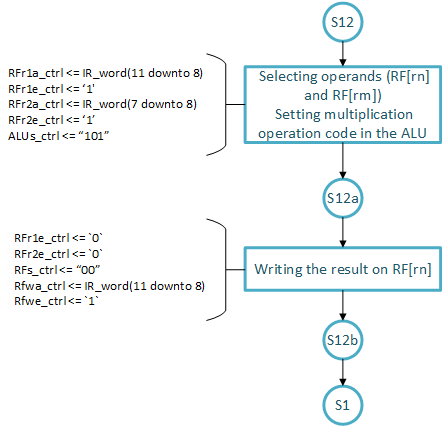
\includegraphics[width=0.45\textwidth]{mult}
	\label{fig:1}
\end{figure}

\begin{lstlisting}[language=vhdl, caption={Multiplication state vhdl}, label={}]
when S12 =>	-- RF[rn] <- RF[rn] * RF[rm]
	RFr1a_ctrl <= IR_word(11 downto 8);	
	RFr1e_ctrl <= '1'; 
	RFr2a_ctrl <= IR_word(7 downto 4);
	RFr2e_ctrl <= '1';  
	ALUs_ctrl <= "101";
	state <= S12a;
when S12a =>   
	RFr1e_ctrl <= '0';
	RFr2e_ctrl <= '0';
	RFs_ctrl <= "00";
	RFwa_ctrl <= IR_word(11 downto 8);
	RFwe_ctrl <= '1';
	state <= S12b;
when S12b =>  
	state <= S1;	
\end{lstlisting}

\subsubsection{Indexed-memory read}

In order to read stored data from the memory, we can count on the instruction \textit{mov1}. Nevertheless, this operation presents two problems. First, we need to specify directly in the instruction the address of the stored element to be read, which means that recursiveness gets too complicated when it comes to several mathematical operations. Second, the limit for addressable locations given by this instruction is 255 or 0xFF, which is a very reduced portion of the reference system's memory. Therefore, it was imperative that a new instruction be designed that can solve these setbacks. By indexing, we can use the CPU registers to set the addresses of the elements that we want to process. In doing so, we can now address $2^{16}-1=65535$ possible locations, which meet the requirements of the reference system. Moreover, the fact that the address can be expressed within the content of a register enables us to use this instruction inside a loop more easily since it can modified after each iteration. The description of the indexed-memory read instruction is as follows:
\begin{table}[h]
	\centering
	{\rowcolors{2}{blue!60!yellow!50}{blue!50!yellow!40}
		\begin{tabular}{|p{3cm}|p{3cm}|p{3.2cm}|}
			\hline
			\textbf{Symbolic} & \textbf{Operation Code} & \textbf{HDL} \\
			\hline
			mov5 & '1001' = 0x9 & RF[$r_m$]$\leftarrow$mem[RF[$r_n$]]\\
			\hline
		\end{tabular}
	}
	%\caption{Multiplication instruction description}
	%\label{tab:2}
\end{table}

The procedure to perform the indexed-memory read is shown in Fig. \ref{fig:2} along with the code.
\begin{figure}[H]
	\caption{Indexed memory read state diagram}
	\centering
	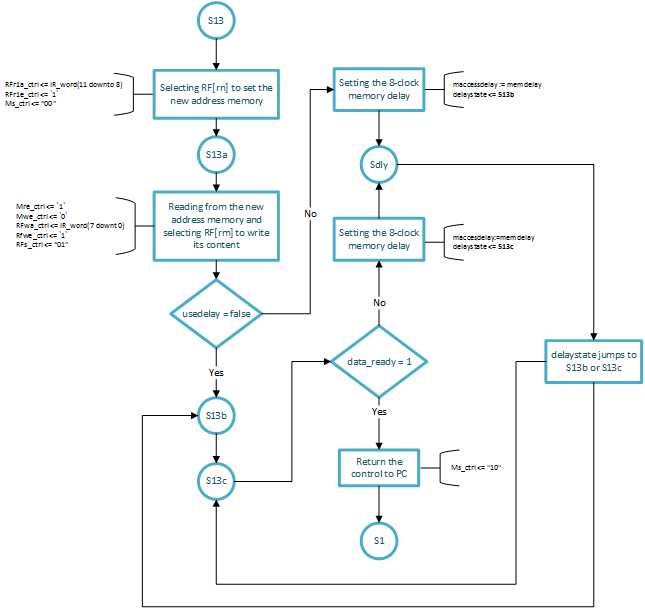
\includegraphics[width=0.78\textwidth]{mov5}
	\label{fig:2}
\end{figure}
\begin{lstlisting}[language=vhdl, caption={Indexed memory read state vhdl}, label={}]
when S13 =>	-- RF[rm] <- mem[RF[rn]]  		 			
	RFr1a_ctrl <= IR_word(11 downto 8);	
	RFr1e_ctrl <= '1';  
	Ms_ctrl <= "00"; -- fetching content of RF[rn] for address memory			
	state <= S13a;
when S13a =>	
	Mre_ctrl <= '1';			
	Mwe_ctrl <= '0';
	RFwa_ctrl <= IR_word(7 downto 4); -- RF[rm]
	RFwe_ctrl <= '1';
	RFs_ctrl <= "01"; -- save mem_data
	if usedelay = false then 
		state <= S13b;
	else 
		maccesdelay := memdelay;
		delaystate <= S13b;
		state <= Sdly;
	end if;										
when S13b => 	
	state <= S13c;
when S13c => 	
	if data_ready = '1' then
		Ms_ctrl <= "10";-- return				
		state <= S1;
	elsif data_ready = '0' then
		maccesdelay := memdelay;
		delaystate <= S13c;
		state <= Sdly;
	end if;
\end{lstlisting}

\subsubsection{Jump if not equal}

The operation \textit{jz} from the original set allows us to control the program flow and implement loops; however, the destination operand is defined by the immediate constant, which is 8-bit long and let us branch only within the first 255 memory locations. In the light of this issue, we dealt with it by setting up a new instruction called \textit{jump if not equal}. The \textit{jump-if-not-equal} operation uses the three registers involved in the instruction format. The first two operands are utilized to verify the condition, which checks if their content are not the same. If the condition yields true then the Program Counter is set to the content of the third register, otherwise the Program Counter behaves regularly. The description of the jump-if-not-equal instruction is as follows:
\begin{table}[h]
	\centering
	{\rowcolors{2}{blue!60!yellow!50}{blue!50!yellow!40}
		\begin{tabular}{|p{3cm}|p{3cm}|p{4.7cm}|}
			\hline
			\textbf{Symbolic} & \textbf{Operation Code} & \textbf{HDL} \\
			\hline
			jne & '1010' = 0xA & if RF[$r_n$]$\neq$RF[$r_m$]:PC$\leftarrow$RF[$r_o$]\\
			\hline
		\end{tabular}
	}
	%\caption{Multiplication instruction description}
	%\label{tab:2}
\end{table}

The procedure to perform the jump-if-not-equal operation is shown in Fig. \ref{fig:3} along with the code.
\begin{figure}[H]
	\caption{Jump if not equal state diagram}
	\centering
	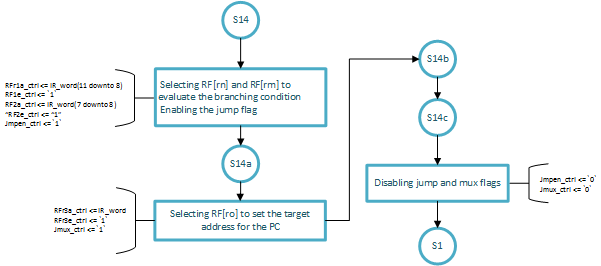
\includegraphics[width=1\textwidth]{jne}
	\label{fig:3}
\end{figure}

\begin{lstlisting}[language=vhdl, caption={Jump if not equal state vhdl}, label={}]
when S14 =>  -- jne, RF[rn] ~= RF[rm] : PC[RF[ro]] 
	RFr1a_ctrl <= IR_word(11 downto 8);	
	RFr1e_ctrl <= '1'; 
	RFr2a_ctrl <= IR_word(7 downto 4);	
	RFr2e_ctrl <= '1'; 					
	jmpen_ctrl <= '1';
	state <= S14a;
when S14a =>   
	RFr3a_ctrl <= IR_word(3 downto 0);	
	RFr3e_ctrl <= '1'; 
	jmux_ctrl	<= '1';
	state <= S14b;
when S14b =>   
	state <= S14c;
when S14c =>   
	jmpen_ctrl <= '0';
	jmux_ctrl	<= '0';
	state <= S1;
\end{lstlisting}

\subsubsection{Increment}

With the original instruction set, two operations has to be executed in order to achieve unitary increments: first, one register has to be set to one and, second, execute the addition instruction with this last register; this makes the code more extensive and less intuitive. Besides, inside a loop, unitary increments are very common. In that sense, we designed the increment instruction which increases by a unit the value of the register specified in the first operand of the instruction format. The description of the increment operation is as follows:
\begin{table}[h]
	\centering
	{\rowcolors{2}{blue!60!yellow!50}{blue!50!yellow!40}
		\begin{tabular}{|p{3cm}|p{3cm}|p{3cm}|}
			\hline
			\textbf{Symbolic} & \textbf{Operation Code} & \textbf{HDL} \\
			\hline
			inc & '1011' = 0xB & RF[$r_n$]$\leftarrow$RF[$r_n$]$+1$\\
			\hline
		\end{tabular}
	}
	%\caption{Multiplication instruction description}
	%\label{tab:2}
\end{table}

The procedure to perform the increment instruction is shown in Fig. \ref{fig:4} along with the code.
\begin{figure}[H]
	\caption{Increment state diagram}
	\centering
	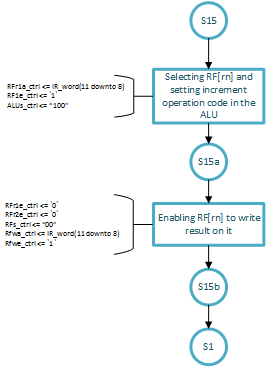
\includegraphics[height=9cm]{inc}
	\label{fig:4}
\end{figure}

\begin{lstlisting}[language=vhdl, caption={Increment state vhdl}, label={}]
when S15 =>	-- inc, RF[rn] <- RF[rn] + 1
	RFr1a_ctrl <= IR_word(11 downto 8);	
	RFr1e_ctrl <= '1'; 
	ALUs_ctrl <= "100";
	state <= S15a;
when S15a =>   
	RFr1e_ctrl <= '0';
	RFr2e_ctrl <= '0';
	RFs_ctrl <= "00";
	RFwa_ctrl <= IR_word(11 downto 8);
	RFwe_ctrl <= '1';
	state <= S15b;
when S15b =>  
	state <= S1;
\end{lstlisting}

\subsubsection{Register-to-register move}

In general terms, it is more efficient to keep the data that has to be processed inside the CPU registers until every calculation that needs it is done. In this way, there is no need to reach the memory, which could take many clock cycles from the CPU. For this reason, it is useful to copy the content from one register to another temporarily, so it can be accessed rapidly without the need to store it to and then retrieve it from the memory. The data movement from one register to another, for our instruction format, copies the content from the second operand to the content of the first operand. The description of the register-to-register move operation is as follows:
\begin{table}[h]
	\centering
	{\rowcolors{2}{blue!60!yellow!50}{blue!50!yellow!40}
		\begin{tabular}{|p{3cm}|p{3cm}|p{3cm}|}
			\hline
			\textbf{Symbolic} & \textbf{Operation Code} & \textbf{HDL}                   \\ \hline
			mov6              & '1100' = 0xC            & RF[$r_n$]$\leftarrow$RF$[r_m]$ \\ \hline
		\end{tabular}
	}
	%\caption{Multiplication instruction description}
	%\label{tab:2}
\end{table}

The procedure to perform the register-to-register move instruction is shown in Fig. \ref{fig:5} along with the code.
\begin{figure}[H]
	\caption{Register-to-register move state diagram}
	\centering
	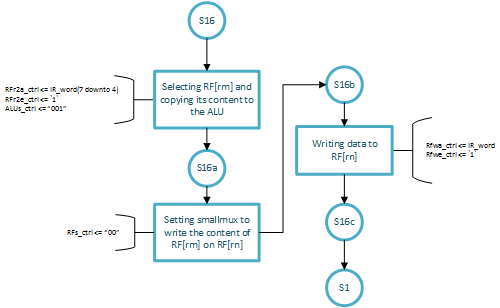
\includegraphics[width=0.7\textwidth]{mov6}
	\label{fig:5}
\end{figure}

\begin{lstlisting}[language=vhdl, caption={Register-to-register move state vhdl}, label={}]
when S16 =>	-- RF[rn] <- RF[rm] 							 
	RFr2a_ctrl <= IR_word(7 downto 4);
	RFr2e_ctrl <= '1';
	ALUs_ctrl <= "001";
	state <= S16a;
when S16a =>
	RFs_ctrl <= "00";				
	state <= S16b;
when S16b =>
	RFwa_ctrl <= IR_word(11 downto 8);
	RFwe_ctrl <= '1';			
	state <= S16c;
when S16c =>
	state <= S1;	
\end{lstlisting}

\subsubsection{Indexed memory out}

The instruction in charge of displaying results (readm) presents the same problem of the instructions that use the immediate constant as part of their execution: the lack of bits to address the whole memory. Taking into consideration this caveat, we designed a instruction that reads the content from the memory indexed by the content of the register specified in the first operand. he description of the register-to-register move operation is as follows:
\begin{table}[h]
	\centering
	{\rowcolors{2}{blue!60!yellow!50}{blue!50!yellow!40}
		\begin{tabular}{|p{3cm}|p{3cm}|p{3cm}|}
			\hline
			\textbf{Symbolic} & \textbf{Operation Code} & \textbf{HDL}                   \\ \hline
			outRF              & '1101' = 0xD            & out$\leftarrow$RF$[r_n]$ \\ \hline
		\end{tabular}
	}
	%\caption{Multiplication instruction description}
	%\label{tab:2}
\end{table}

The procedure to perform the register-to-register move instruction is shown in Fig. \ref{fig:6} along with the code.

\begin{figure}[H]
	\caption{Indexed memory out state diagram}
	\centering
	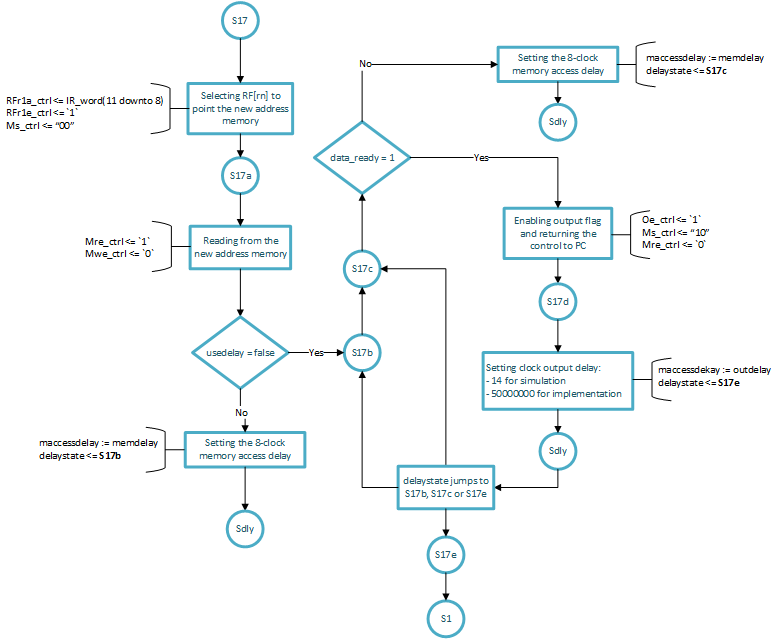
\includegraphics[width=1\textwidth]{outRF}
	\label{fig:6}
\end{figure}

\begin{lstlisting}[language=vhdl, caption={Indexed memory out state vhdl}, label={}]
when S17 => -- output <- mem[RF[rn]]   
	RFr1a_ctrl <= IR_word(11 downto 8);	
	RFr1e_ctrl <= '1';  
	Ms_ctrl <= "00"; -- selecting content of RFr1 for address memory					
	state <= S17a;				
when S17a => 
	Mre_ctrl <= '1'; -- read memory
	Mwe_ctrl <= '0';
	if usedelay = false then 
		state <= S17b;
	else 
		maccesdelay := memdelay;
		delaystate <= S17b;
		state <= Sdly;
	end if;
when S17b =>					
	state <= S17c;
when S17c =>
	if data_ready = '1' then
		oe_ctrl <= '1';
		Ms_ctrl <= "10"; -- return				
		Mre_ctrl <= '0';
		state <= S17d;
	elsif data_ready = '0' then
		maccesdelay:=memdelay;
		delaystate <= S17c;
		state <= Sdly;
	end if;
when S17d =>
	maccesdelay:=outdelay;
	delaystate <= S17e;
	state <= Sdly;
when S17e => 
	state <= S1;
\end{lstlisting}

\subsubsection{Reference system's instruction set}

After the implementation of the instructions described before, a new instruction set was created which is shown in Table \ref{tab:2}.

\begin{table}[!ht]
	\centering
	{\rowcolors{3}{green!80!yellow!50}{green!70!yellow!40}
	\begin{tabular}{|p{1.5cm}|p{2.8cm}|p{4.7cm}|}
		\hline
		\multicolumn{3}{|c|}{\textbf{Reference Instruction Set}} \\
		\hline
		\textbf{Symbolic} & \textbf{Operation Code} & \textbf{HDL} \\
		\hline
		mov1 & '0000' = 0x0 & RF[$r_n$]$\leftarrow$mem[direct]\\
		mov2 & '0001' = 0x1 & mem[direct]$\leftarrow$RF[$r_n$]\\
		mov3 & '0010' = 0x2 & mem[RF[$r_n$]]$\leftarrow$RF[$r_m$]\\
		mov4 & '0011' = 0x3 & RF[$r_n$]$\leftarrow$imm\\
		add & '0100' = 0x4 & RF[$r_n$]$\leftarrow$RF[$r_n$]$+$RF[$r_m$]\\
		subt & '0101' = 0x5 & RF[$r_n$]$\leftarrow$RF[$r_n$]$-$RF[$r_m$]\\
		jz & '0110' = 0x6 & if RF[$r_n$]$=0$:PC$\leftarrow$imm\\
		readm & '0111' = 0x7 & out$\leftarrow$mem[direct]\\
		mult & '1000' = 0x8 & RF[$r_n$]$\leftarrow$RF[$r_n$]$*$RF[$r_m$]\\
		mov5 & '1001' = 0x9 & RF[$r_m$]$\leftarrow$mem[RF[$r_n$]]\\
		jne & '1010' = 0xA & if RF[$r_n$]$\neq$RF[$r_m$]:PC$\leftarrow$RF[$r_o$]\\
		inc & '1011' = 0xB & RF[$r_n$]$\leftarrow$RF[$r_n$]$+1$\\
		mov6 & '1100' = 0xC & RF[$r_n$]$\leftarrow$RF$[r_m]$ \\
		outRF & '1101' = 0xD & out$\leftarrow$RF$[r_n]$ \\
		halt & '1111' = 0xF & do nothing \\
		\hline
	\end{tabular}
	}
	\caption{Reference system's instruction set}
	\label{tab:2}
\end{table}

\subsection{Cache implementation}

\subsubsection{Memory organization}

The reference main memory size is 4 kbytes of 16 bits words (address width of 12 \footnote{Review subsection \ref{error} (Unexpected compilation error) to know the reason why we changed from 12-bit address to 11-bit address.}
bits) while the enhanced system requires that the memory be a two-level memory with a slow (main) memory size of 4kbytes with 64-bit lines and a total of 1024 lines and fast (cache) memory with 32 words of 16 bits organized in 8 lines of 4
words per line. Taking into account these requirements, the organization of the enhanced memory in contrast with the organization of the reference memory are shown in Fig. \ref{fig:7}.

\begin{figure}[!ht]
	\caption{Memory organization of the reference and enhanced systems}
	\centering
	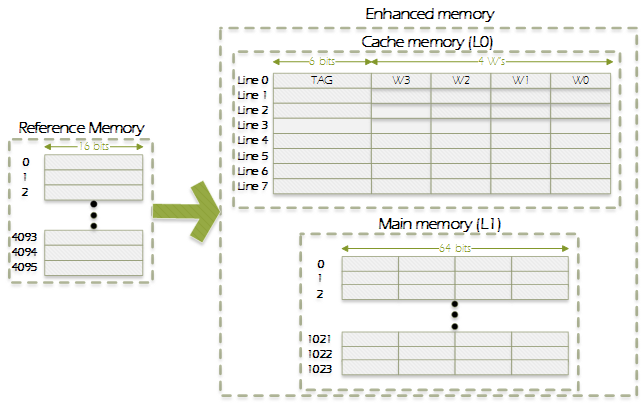
\includegraphics[width=0.7\textwidth]{memory}
	\label{fig:7}
\end{figure}

\subsubsection{Data transfer}

In order to execute a program or application, the CPU sends directions to the enhanced memory asking for data words to process and, hopefully, that information is in the cache memory which is very fast and can satisfy the CPU's processing speed needs. However, if the information is not inside the cache, then some mechanism must be executed so that the required data gets to the CPU. This mechanism is the cache controller and its main purpose is make sure that the data required be inside the cache. Therefore, the cache controller is in charge of the data transfer between the enhanced memory and the CPU.

When the CPU asks for data that is not found in the cache memory, the cache controller retrieves the information from the main memory, but the transfer between the cache and the main memory is done by blocks. The reason to do that is based on the principle of locality, which assumes that most probably the next data word that will be required is inside the block that was transfered to the cache. In this way, there is no need to reach the main memory slowing down the program execution. Fig. \ref{fig:8} shows the transfers performed in the system.

\begin{figure}[H]
	\caption{Data transfer diagram}
	\centering
	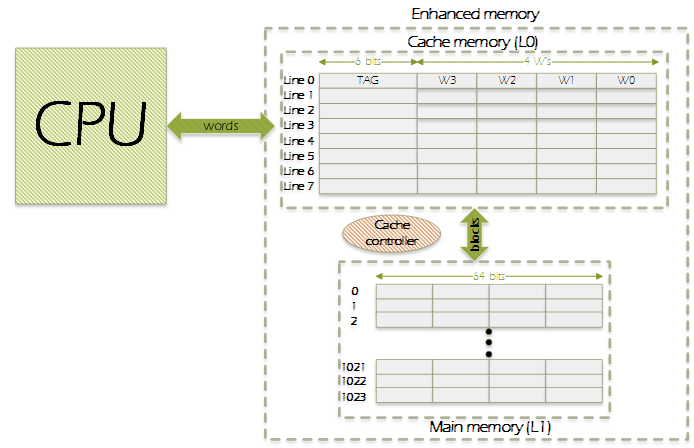
\includegraphics[width=0.7\textwidth]{cpu_memory}
	\label{fig:8}
\end{figure}

\subsubsection{Cache controller}

Determining if the required data word is in the cache is, as well, one of functions that the cache controller must perform and it is achieved by analyzing the address direction set by the CPU. The first operation is to point to one of the eight lines of the cache using the line field (bits 3 to 5) extracted from the address. After that, the tag fields from the line and from the address (bits 6 to 12) are compared in order to know if they are the same. If they are equal then it is a hit and the data word in the line that is going to be transfered is selected by the word field in the address (bits 1 to 2). Otherwise, it is a miss, which means that the block in the selected line has to be moved to the main memory and a new block with the required data from the main memory has to take this position. This procedures takes eight clock cycles for purposes of simulation. Finally, once the data is already in the cache, the needed word is chosen with the word field and then it is sent to the CPU. Fig. \ref{fig:9} illustrates how the cache establishes if the required information is or is not in the cache memory and Fig. \ref{fig:10} and Fig. \ref{fig:11} shows the complete operation of the cache controller.

\begin{figure}[H]
	\caption{Cache controller operation}
	\centering
	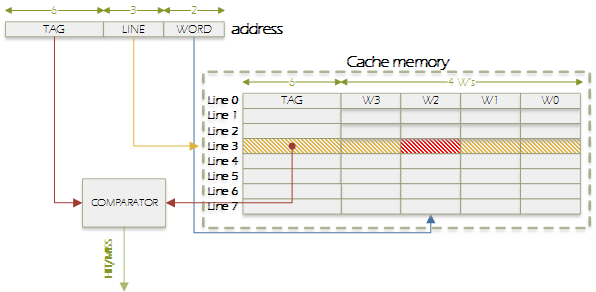
\includegraphics[width=0.7\textwidth]{Direct_mapping}
	\label{fig:9}
\end{figure}

\begin{figure}[H]
	\caption{Cache controller initial and reading operation }
	\centering
	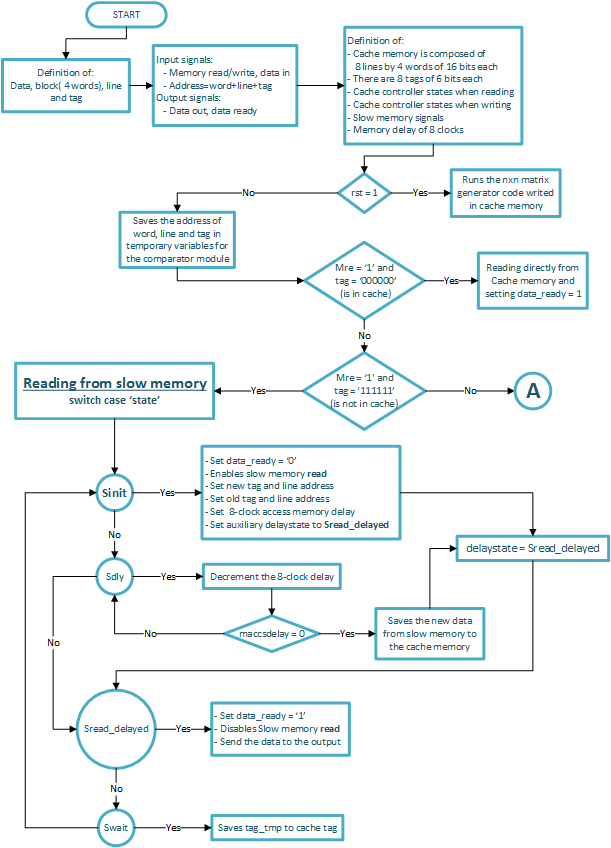
\includegraphics[width=0.9\textwidth]{cache_controller_a}
	\label{fig:10}
\end{figure}

\begin{figure}[H]
	\caption{Cache controller writing operation}
	\centering
	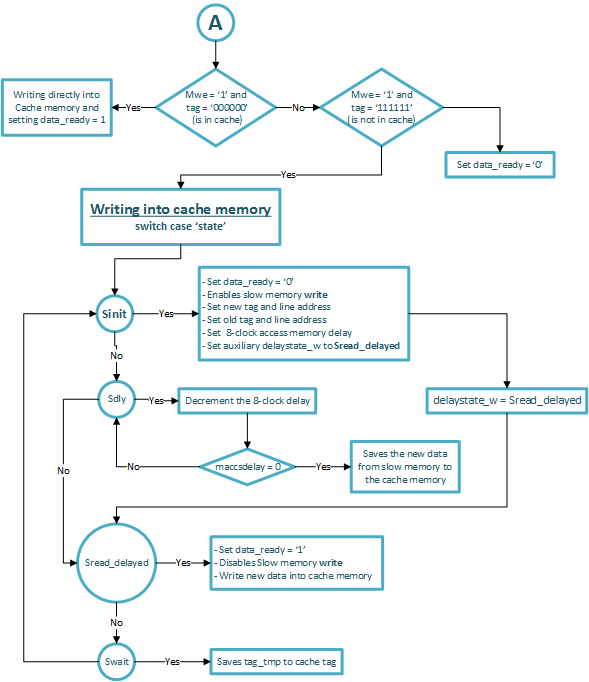
\includegraphics[width=0.9\textwidth]{cache_controller_b}
	\label{fig:11}
\end{figure}

\begin{lstlisting}[language=vhdl, caption={Cache controller vhdl}, label={}]
process(clock, rst, Mwe, Mre, address, data_in, state)
	variable word_tmp: std_logic_vector((block_size)-1 downto 0);	
	variable line_tmp:std_logic_vector((line_size)-1 downto 0);
	variable tag_tmp: std_logic_vector((tag_size)-1 downto 0);
	variable maccesdelay: integer;
	begin
	if rst='1' then					
		--	A&B nxn matrix generator (vhdl)
			
		data_out <= ZERO;
		state <= Sinit;
		state_W <= Sinit;
	elsif (clock'event and clock = '1') then
		word_tmp := address(block_size-1 downto 0);
		line_tmp := address((block_size+line_size)-1 downto block_size);
		tag_tmp := address((block_size+line_size+tag_size)-1 downto (block_size+line_size));
	
		-- Reading directly from Cache memory
		if (Mre ='1' and Mwe ='0' and tag_tmp = cache_tag(conv_integer(line_tmp))) then
			data_ready <= '1';		
			data_out <= tmp_ram(conv_integer(line_tmp),conv_integer(word_tmp));
		
		-- Reading from slow memory
		elsif (Mre ='1' and Mwe ='0' and tag_tmp /= cache_tag(conv_integer(line_tmp))) then	
			case state is
				when Sinit =>
					data_ready <= '0';
					SM_rw_enable <= '1';
					new_address((tag_size+line_size)-1 downto (line_size)) <= tag_tmp;
					new_address((line_size-1) downto 0) <= line_tmp;
					old_address((tag_size+line_size)-1 downto (line_size)) <= cache_tag(conv_integer(line_tmp));
					old_address((line_size-1) downto 0) <= line_tmp;
					old_data <= tmp_ram(conv_integer(line_tmp),0) & tmp_ram(conv_integer(line_tmp),1) & tmp_ram(conv_integer(line_tmp),2) & tmp_ram(conv_integer(line_tmp),3);
					maccesdelay:=memdelay;
					delaystate <= Sread_delayed;
					state <= Sdly;
				when Sdly =>								-- Delay State	
					maccesdelay := maccesdelay-1;
					if maccesdelay = 0 then 
						tmp_ram(conv_integer(line_tmp),0) <= new_data((data_width*(2**block_size))-1 downto (data_width*(2**block_size-1)));
						tmp_ram(conv_integer(line_tmp),1) <= new_data((data_width*(2**block_size-1))-1 downto (data_width*(2**block_size-2)));
						tmp_ram(conv_integer(line_tmp),2) <= new_data((data_width*(2**block_size-2))-1 downto (data_width*(2**block_size-3)));
						tmp_ram(conv_integer(line_tmp),3) <= new_data((data_width*(2**block_size-3))-1 downto 0);
						state <= delaystate;
					else 
						state <= Sdly ;
					end if;
				when Sread_delayed =>
					data_ready <= '1';
					SM_rw_enable <= '0';
					data_out <= tmp_ram(conv_integer(line_tmp),conv_integer(word_tmp));
					state <= Swait;
				when Swait =>
					cache_tag(conv_integer(line_tmp)) <= tag_tmp;
					state <= Sinit;
			end case;
		
		-- Writing into cache memory	
		elsif (Mwe ='1' and Mre = '0' and tag_tmp = cache_tag(conv_integer(line_tmp))) then
			data_ready <= '1';
			tmp_ram(conv_integer(line_tmp),conv_integer(word_tmp)) <= data_in;
		elsif (Mwe ='1' and Mre = '0' and tag_tmp /= cache_tag(conv_integer(line_tmp))) then		
			case state_w is
				when Sinit =>
					data_ready <= '0';
					SM_rw_enable <= '1';
					new_address((tag_size+line_size)-1 downto (line_size)) <= tag_tmp;
					new_address((line_size-1) downto 0) <= line_tmp;
					old_address((tag_size+line_size)-1 downto (line_size)) <= cache_tag(conv_integer(line_tmp));
					old_address((line_size-1) downto 0) <= line_tmp;
					old_data <= tmp_ram(conv_integer(line_tmp),0) & tmp_ram(conv_integer(line_tmp),1) & tmp_ram(conv_integer(line_tmp),2) & tmp_ram(conv_integer(line_tmp),3);
					maccesdelay:=memdelay;
					delaystate_w <= Sread_delayed;
					state_w <= Sdly;
				when Sdly =>								-- Delay State	
					maccesdelay := maccesdelay-1;
					if maccesdelay = 0 then 
						tmp_ram(conv_integer(line_tmp),0) <= new_data((data_width*(2**block_size))-1 downto (data_width*(2**block_size-1)));
						tmp_ram(conv_integer(line_tmp),1) <= new_data((data_width*(2**block_size-1))-1 downto (data_width*(2**block_size-2)));
						tmp_ram(conv_integer(line_tmp),2) <= new_data((data_width*(2**block_size-2))-1 downto (data_width*(2**block_size-3)));
						tmp_ram(conv_integer(line_tmp),3) <= new_data((data_width*(2**block_size-3))-1 downto 0);
						state_w <= delaystate_w;
					else 
						state_w <= Sdly ;
					end if;
				when Sread_delayed =>
					data_ready <= '1';
					SM_rw_enable <= '0';
					tmp_ram(conv_integer(line_tmp),conv_integer(word_tmp)) <= data_in;
					state_w <= Swait;
				when Swait =>
					cache_tag(conv_integer(line_tmp)) <= tag_tmp;
					state_w <= Sinit;
			end case;		
		else
			data_ready <= '0';		
		end if;
	end if;
end process;
Unit: memory_slow port map(clock,rst,SM_rw_enable,old_address,new_address,old_data,new_data);
\end{lstlisting}

\subsection{Program design}

\subsubsection{Matrix generator}
The dimension of the two matrices that we have to operate are 10x10, which means that every matrix has 100 elements. Therefore, we can set every single element manually or we can generate them automatically. Since it takes two instructions to store an element, we will need 400 instructions to store all the matrices elements. This last procedure is too tedious. Instead, we generated the matrices element with a short algorithm that produces a first matrix with even numbers and a second matrix with odd numbers interleaved with zeros so that the results do not exceed the maximum register value (65535). The matrices are the following:

\[
	A=
	\begin{bmatrix}
	0 & 0 & 2 & 0 & 4 &  \dots  \\
	10 & 0 & 12 & 0 & 14 & \dots  \\
	20 & 0 & 22 & 0 & 24 & \dots  \\
	30 & 0 & 32 & 0 & 34 & \dots  \\
	40 & 0 & 42 & 0 & 44 & \dots  \\
	\vdots & \vdots & \vdots & \vdots & \vdots & \ddots \\
	\end{bmatrix}_{10x10},
	B=
	\begin{bmatrix}
	1 & 0 & 3 & 0 & 5 &  \dots  \\
	11 & 0 & 13 & 0 & 15 & \dots  \\
	21 & 0 & 23 & 0 & 25 & \dots  \\
	31 & 0 & 33 & 0 & 35 & \dots  \\
	41 & 0 & 43 & 0 & 45 & \dots  \\
	\vdots & \vdots & \vdots & \vdots & \vdots & \ddots \\
	\end{bmatrix}_{10x10}
\]

\begin{figure}[H]
	\caption{Matrix generation algorithm}
	\centering
	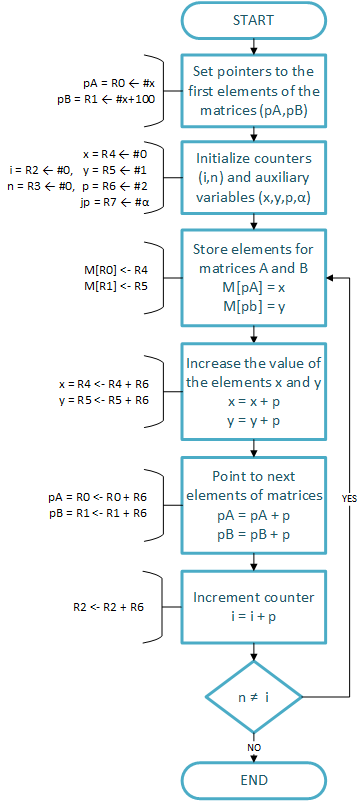
\includegraphics[width=0.5\textwidth]{gen_algorithm}
	\label{fig:12}
\end{figure}

\begin{lstlisting}[language=vhdl, caption={Matrix generator vhdl}, label={}]
--	------------------------------------------------
--	-- A&B nxn matrix generator
--	0 => x"3064" & x"31C8" & x"3200" & x"3364",
--	-- 0:  R0 <- #100 	:pA = 100
--	-- 1:  R1 <- #200 	:pB = 200
--	-- 2:  R2 <- #0		:i = 0
--	-- 3:  R3 <- #100		:n = 100, total matrix elements
--	1 => x"3400" & x"3501" & x"3602" & x"3708", 
--	-- 4:  R4 <- #0		:x = 0
--	-- 5:  R5 <- #1		:y = 1
--	-- 6:  R6 <- #2		:p = 2
--	-- 7:  R7 <- #8(jump position)
--	2 => x"2040" & x"2150" & x"4460" & x"4560",
--	-- 8:  M[R0] <- R4 	:M[pA] = x
--	-- 9:  M[R1] <- R5 	:M[pb] = y
--	-- 10: R4 <- R4 + R6	:x = x + p
--	-- 11: R5 <- R5 + R6	:y = y + p
--	3 => x"4060" & x"4160" & x"4260" & x"A237",
--	-- 12: R0 <- R0 + R6	:pA = pA + p
--	-- 13: R1 <- R1 + R6	:pB = pB + p
--	-- 14: R2 <- R2 + R6	:i = i + p
--	-- 15: R2~=R3:PC<-[R7]  goto([R7]) if R2~=R3		
--			
------------------------------------------------
-- A&B nxn matrix generator
-- tag 0							-- line 0, words 0-3
cache_tag(0) <= "000000";	tmp_ram(0,0) <= x"3064";tmp_ram(0,1) <= x"31C8";tmp_ram(0,2) <= x"3200";tmp_ram(0,3) <= x"3364";						
-- tag 1							-- line 1, words 4-7
cache_tag(1) <= "000000";	tmp_ram(1,0) <= x"3400";tmp_ram(1,1) <= x"3501";tmp_ram(1,2) <= x"3602";tmp_ram(1,3) <= x"3708";			
-- tag 2							-- line 2, words 8-11
cache_tag(2) <= "000000";	tmp_ram(2,0) <= x"2040";tmp_ram(2,1) <= x"2150";tmp_ram(2,2) <= x"4460";tmp_ram(2,3) <= x"4560";			
-- tag 3							-- line 3, words 12-15
cache_tag(3) <= "000000";	tmp_ram(3,0) <= x"4060";tmp_ram(3,1) <= x"4160";tmp_ram(3,2) <= x"4260";tmp_ram(3,3) <= x"A237";						
-- tag 4							-- line 4, words 16-19
cache_tag(4) <= "111111";			
-- tag 5							-- line 5, words 20-23
cache_tag(5) <= "111111";			
-- tag 6							-- line 6, words 24-27
cache_tag(6) <= "111111";			
-- tag 7							-- line 7, words 28-31
cache_tag(7) <= "111111";			
\end{lstlisting}

\subsubsection{Matrix multiplication}
Considering that the two matrices are stored consecutively, the following algorithm performs the matrix multiplication:
\begin{figure}[H]
	\caption{Multiplication algorithm}
	\centering
	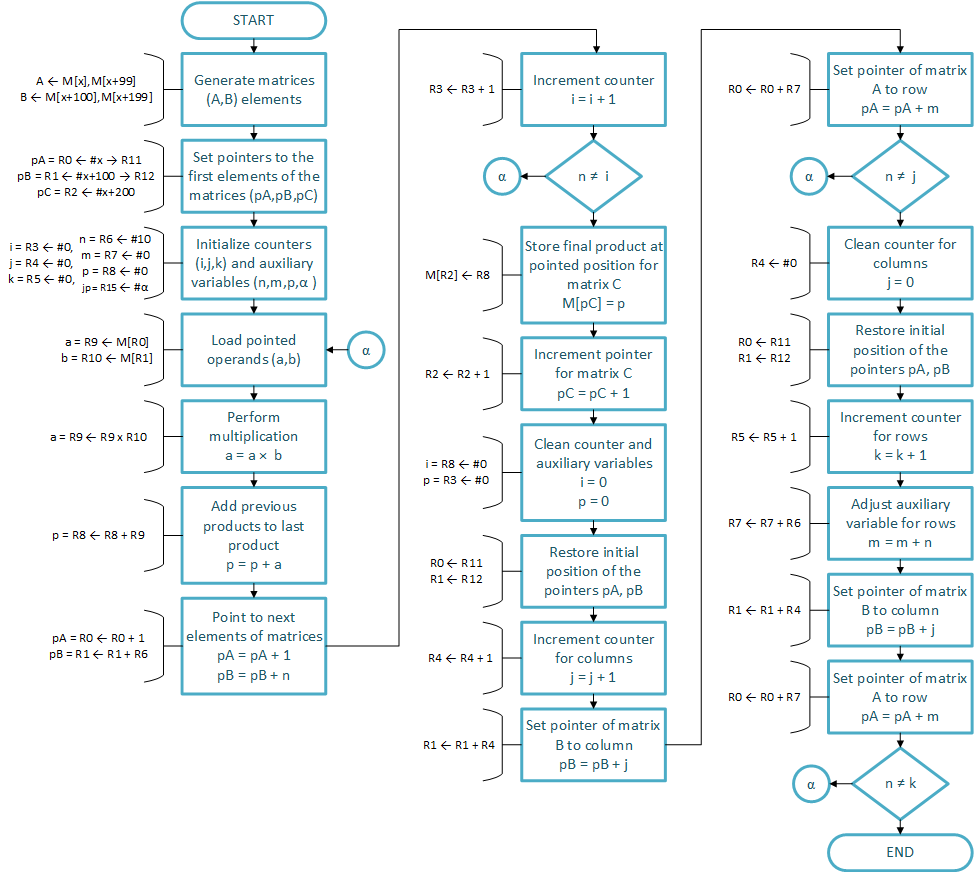
\includegraphics[width=1\textwidth]{mult_algorithm}
	\label{fig:13}
\end{figure}

\begin{lstlisting}[language=vhdl, caption={Matrix multiplication vhdl}, label={}]
-- Matrix multiplication A*B=C
4 => x"3064" & x"3B64" & x"31C8" & x"3CC8",
-- 16: R0  <- #x=100	:pA	
-- 17: R11 <- #x=100		
-- 18: R1  <- #x=200	:pB
-- 19: R12 <- #x=200
5 => x"C210" & x"4200" & x"3300" & x"3400",						
-- 20: R2 <- R1		:#200	  
-- 21: R2 <- R2+R0	:#200+100=300	:pC						
-- 22: R3 <- #0		:i=0
-- 23: R4 <- #0		:j=0						
6 => x"3500" & x"360A" & x"3700" & x"3800",
-- 24: R5 <- #0		:k=0
-- 25: R6 <- #10		:n=10, column number		
-- 26: R7 <- #0		:m=0
-- 27: R8 <- #0		:p=0						
7 => x"3F1D" & x"9090" & x"91A0" & x"89A0",
-- 28: R15 <- #29   	:jp (#alpha)						
-- 29: R9  <- M[R0] 	:a												
-- 30: R10 <- M[R1] 	:b												
-- 31: R9 <- R9*R10 	:a=a*b										
8 => x"4890" & x"B000" & x"4160" & x"B300",
-- 32: R8 <- R8+R9  	:p=p+a										
-- 33: R0 <- R0+1  	:pA=pA+1									
-- 34: R1 <- R1+R6 	:pB=pB+n											
-- 35: R3 <- R3+1  	:i=i+1											
9 => x"A63F" & x"2280" & x"B200" & x"3800",
-- 36: R6~=R3:PC<-[R15]  goto([R15]) if R6~=R3	:n~=i									
-- 37: M[R2] <- R8	:M[pC]=p, store final product						
-- 38: R2 <- R2+1		:pC=pC+1											
-- 39: R8 <- #0		:i=0												
10 => x"3300" & x"C0B0" & x"C1C0" & x"B400",
-- 40: R3 <- #0		:p=0											
-- 41: R0 <- R11		:Restore init pos of pA					
-- 42: R1 <- R12		:Restore init pos of pB						
-- 43: R4 <- R4+1		:j=j+1											
11 => x"4140" & x"4070" & x"A64F" & x"3400",
-- 44: R1 <- R1+R4	:pB=pB+j												
-- 45: R0 <- R0+R7	:pA=pA+m												
-- 46: R6~=R4:PC<-[R15]  goto([R15]) if R6~=R4	:n~=j						
-- 47: R4 <- #0		:j=0
12 => x"C0B0" & x"C1C0" & x"B500" & x"4760",
-- 48: R0 <- R11		:Restore init pos of pA						
-- 49: R1 <- R12		:Restore init pos of pB
-- 50: R5 <- R5+1		:k=k+1, inc row counter
-- 51: R7 <- R7+R6	:m=m+n
13 => x"4140" & x"4070" & x"A65F" & x"3200",
-- 52: R1 <- R1+R4	:pB=pB+j						
-- 53: R0 <- R0+R7	:pA=pA+m						
-- 54: R6~=R5:PC<-[R15]  goto([R15]) if R6~=R5	:n~=k						
-- 55: R2 <- #0			:i=0

-- Output matrix C
14 => x"3364" & x"343D" & x"3564" & x"30C8",												
-- 56: R3 <- #100			:n=100, total matrix elements
-- 57: R4 <- #61(jump position)
-- 58: R5 <- #100	
-- 59: R0 <- #200 				
15 => x"4050" & x"D000" & x"B000" & x"B200",						
-- 60: R0 <- R0+R5		:#300	pA=300
-- 61: output<- M[R0]
-- 62: R0 <- R0+1			:pA=pA+1
-- 63: R2 <- R2+1			:i=i+1
16 => x"A234" & x"F000" & x"0000" & x"0000",						
-- 64: R2~=R3:PC<-[R4]  goto([R4]) if R2~=R3
-- 65: halt		
\end{lstlisting}


\section{Results}
\subsection{Matlab code}
In order to verify the simulation and implementation results, the following code in \verb|matlab| allows us to view the 100 elements of the resultant matrix $A*B = C$, Fig. \ref{fig:matlab}.

\begin{lstlisting}[language=matlab, caption={Matlab multiplication.}, label={}]
clear all; clc; close all;
n=10; % nxn, n value of matrix
x=0; y=1;
for i=1:n 
	for j=1:n
		if mod(j, 2) == 0 	% j is even
			A(i,j)=0;
			B(i,j)=0;
		else                % j is odd
			A(i,j)=x;
			x=x+2;
			B(i,j)=y;
			y=y+2;
		end		
	end
end
A
B
C=A*B
\end{lstlisting} 

\begin{figure}[H]
	\centering
	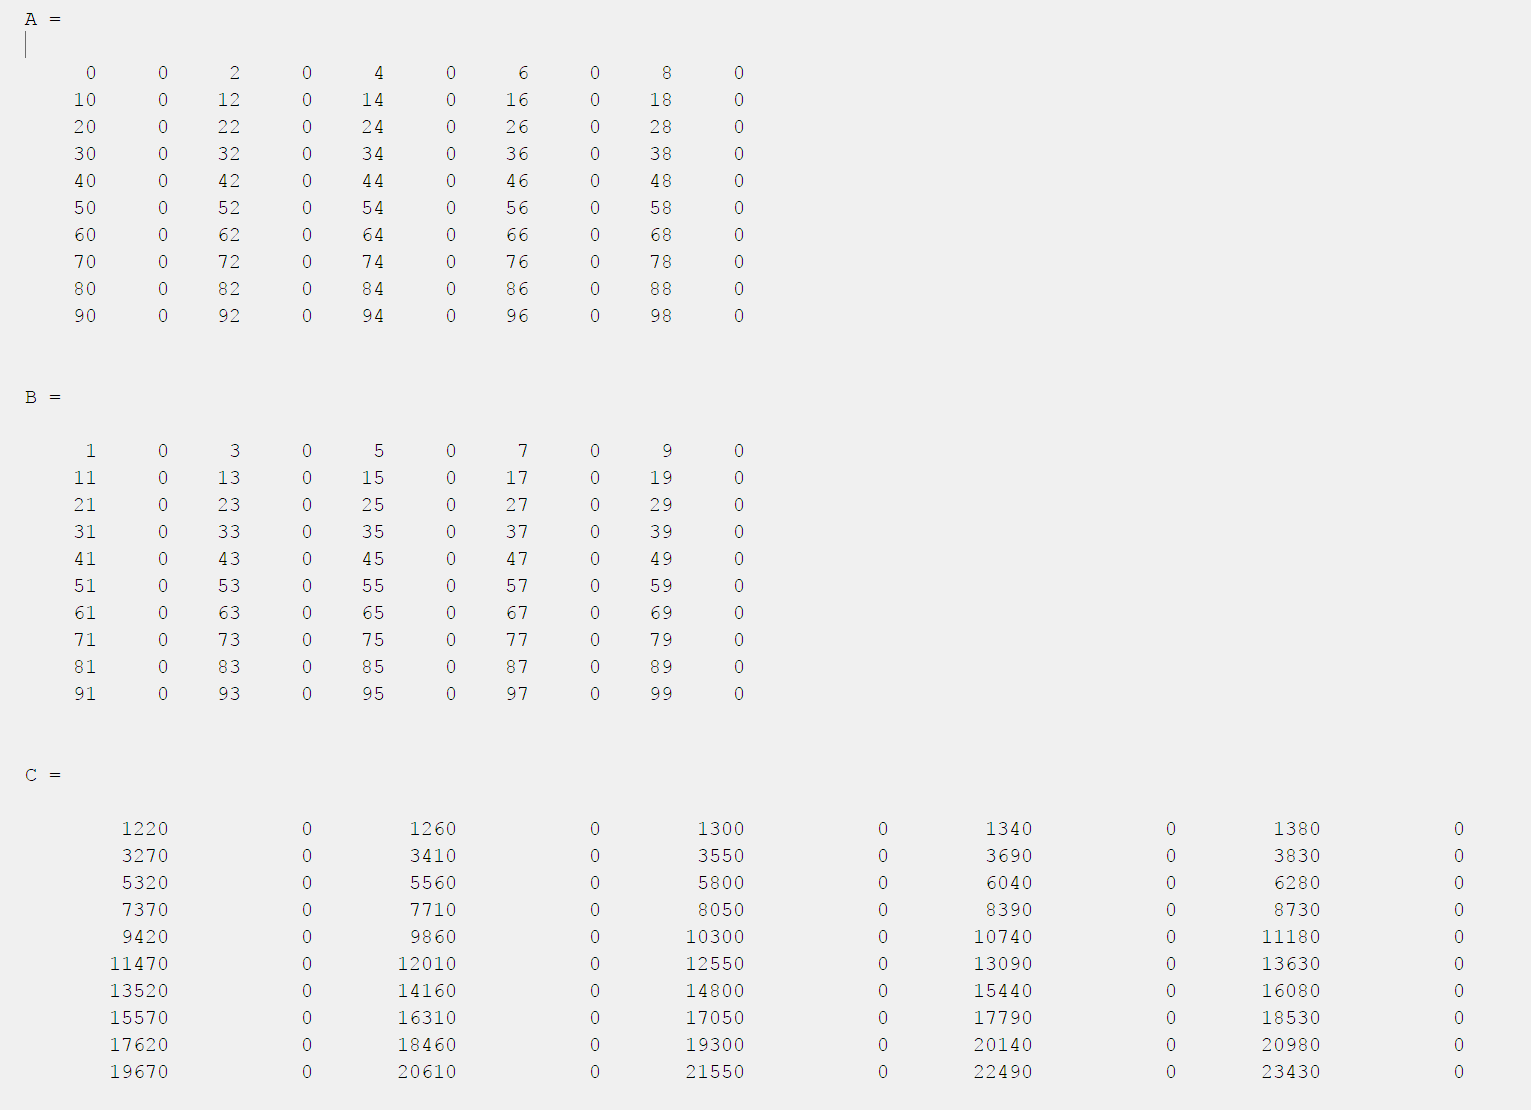
\includegraphics[width=0.8\textwidth]{10x10_matrix_mult}
	\caption{Matlab multiplication.}
	\label{fig:matlab}
\end{figure}

\subsection{Compilation instructions}\label{comp}
Because we are using the same project to test the upgraded performance of the direct mapped cache system vs the use of simple memory system, we need to change some parameters to compile both cases.

\subsubsection*{Cache and simple memory simulation/implementation:}
\begin{enumerate}
	\item Comment/uncomment in \verb|SimpleCompArch.vhd| (line \verb|85-86|) as the following code. 
	\begin{lstlisting}[language=vhdl, caption={}, label={}]
	Unit2: memory port map(sys_clk,sys_rst,Mre,Mwe,mem_addr,mdin_bus,mdout_bus,data_ready); 
	--Unit5: memory_simple port map(sys_clk,sys_rst,Mre,Mwe,mem_addr,mdin_bus,mdout_bus,data_ready);\end{lstlisting}
	\item Edit \verb|controller.vhd| (line \verb|52-53|) with the following values,  
	\begin{lstlisting}[language=vhdl, caption={}, label={}]
	constant outdelay: integer := 50000000; -- 50000000 = 1sec for implementation, 14 for simulation
	signal usedelay: boolean := false; 		-- false for cache memory, true for memory_slow \end{lstlisting}
\end{enumerate} 

\subsection{Cache memory simulation}
Fig. \ref{fig:cache1}a shows the initialization of the whole process, at the same, it can be seen the execution of the First and Second Block in Cache memory, Fig. \ref{fig:cache1}b shows the execution of the Last Block in Cache and the First Block in Slow Memory, during that time the cache controller enters in execution.  

\begin{figure}[H]
	\centering
	\subfigure[Initialization of simulation.]{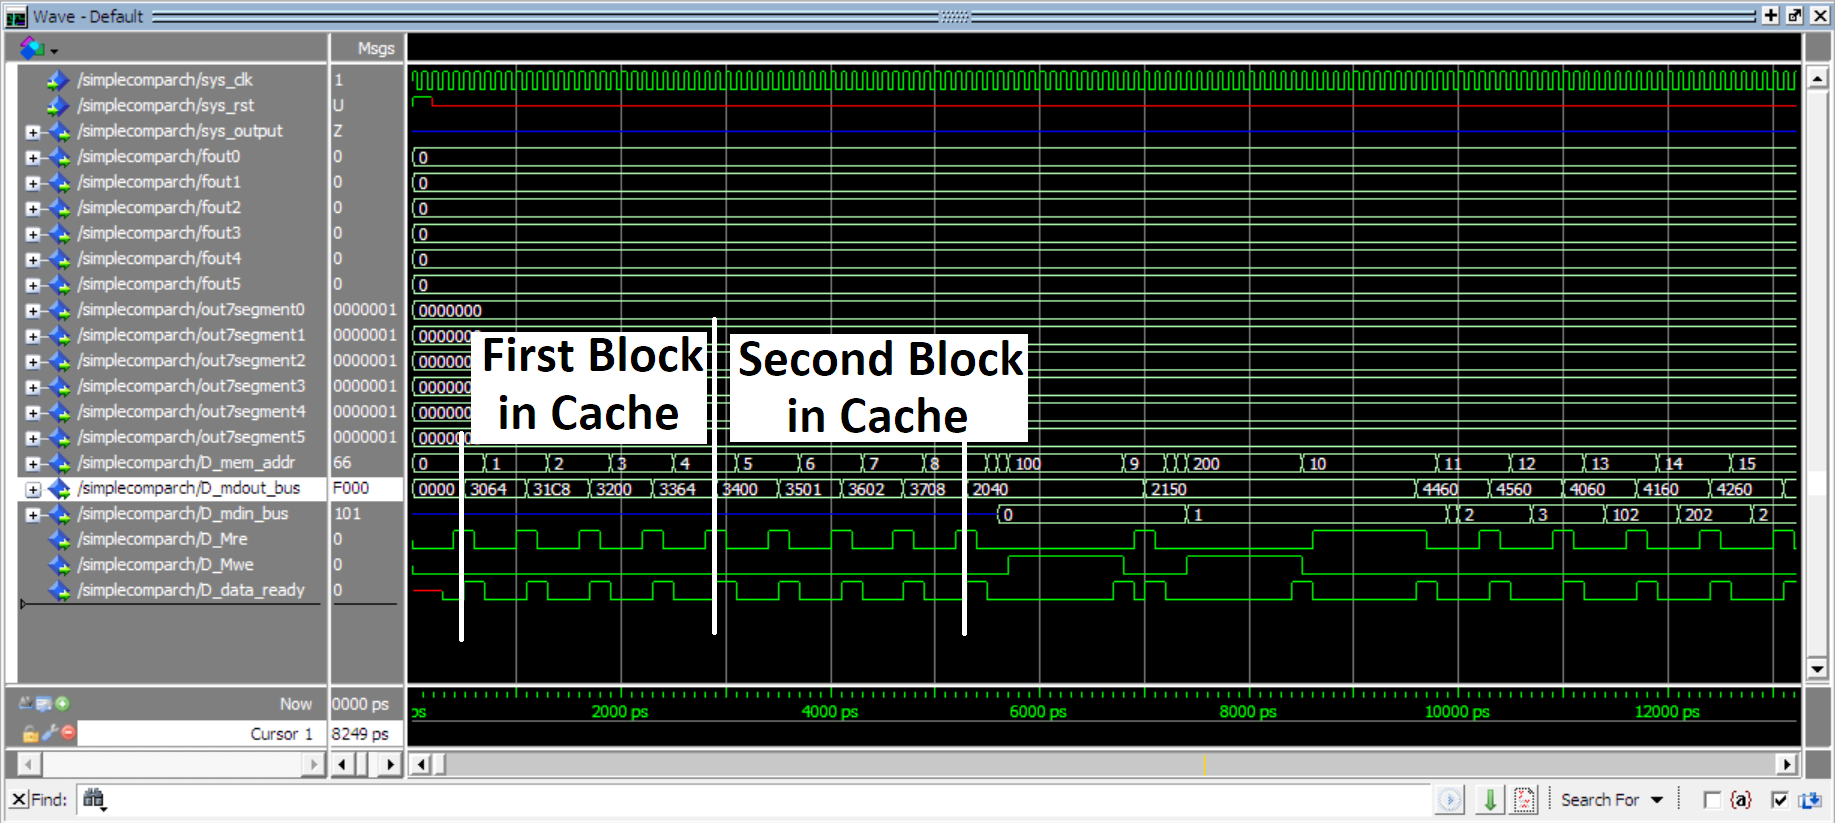
\includegraphics[width=1\linewidth]{./cache/ini_all}}
	\subfigure[Last Block executed in Cache memory and first Block executed in Slow Memory.]{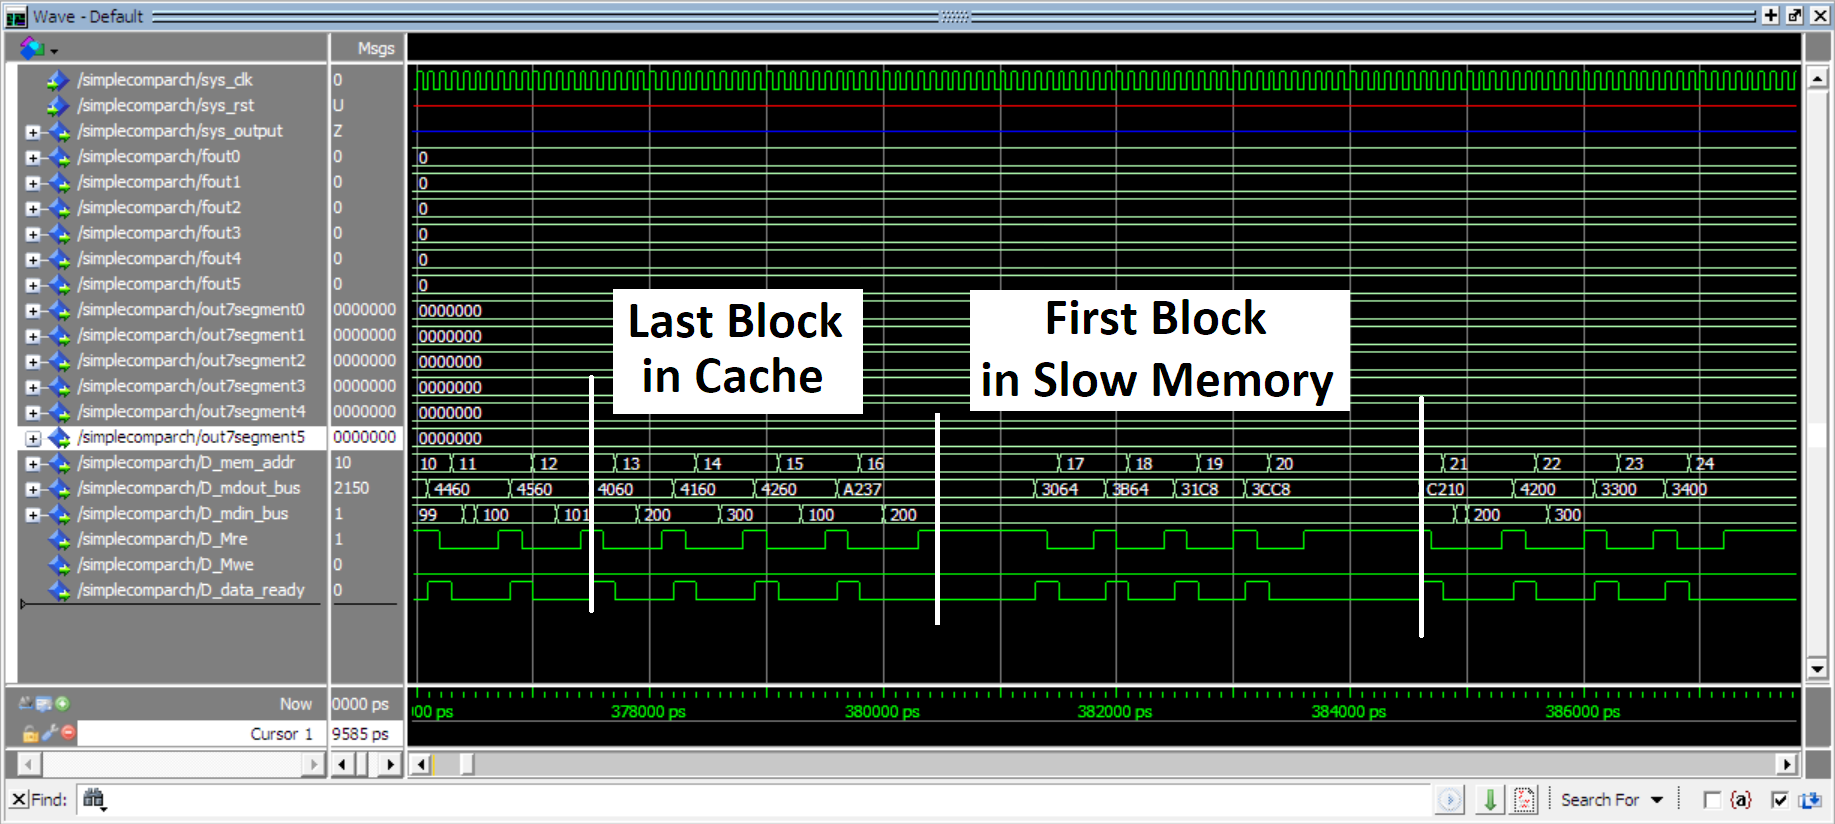
\includegraphics[width=1\linewidth]{./cache/last_line_in_cache_first_memoryslow}}		
	\caption{Cache memory simulation.}
	\label{fig:cache1}
\end{figure}

\subsection{Cache controller execution}
Fig. \ref{fig:cache2}a represents in detail the states of \textbf{Reading from slow memory} process, and Fig. \ref{fig:cache2}b describes the \textbf{Writing into cache memory} process.

\begin{figure}[H]
	\centering
	\subfigure[Reading from slow memory.]{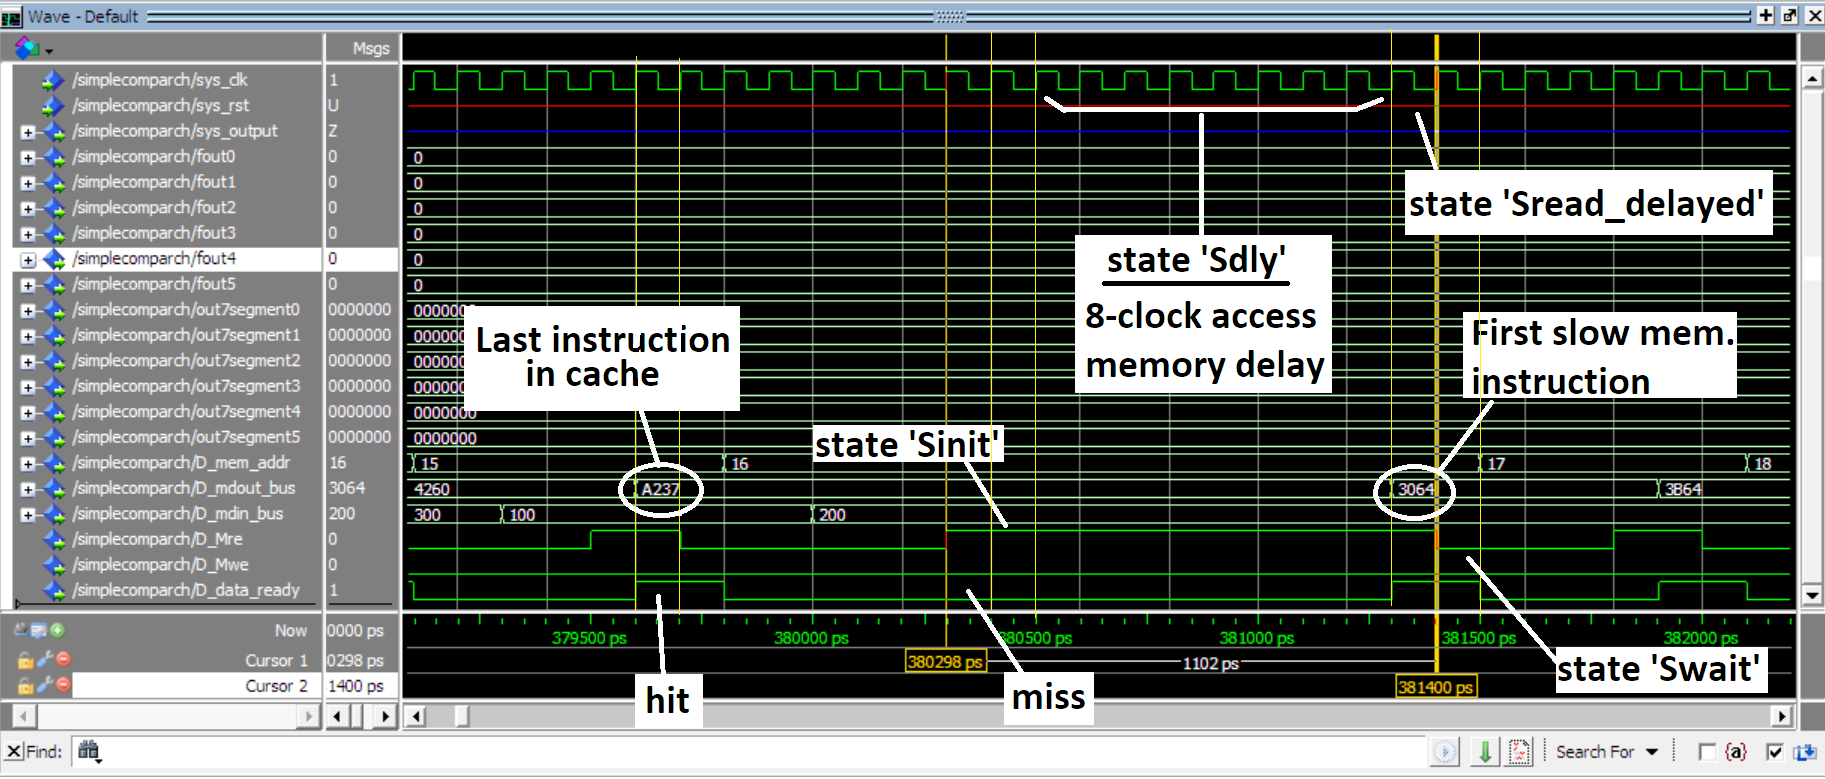
\includegraphics[width=1\linewidth]{./cache/reading_from_slow_memory}}
	\subfigure[Writing into cache memory. ]{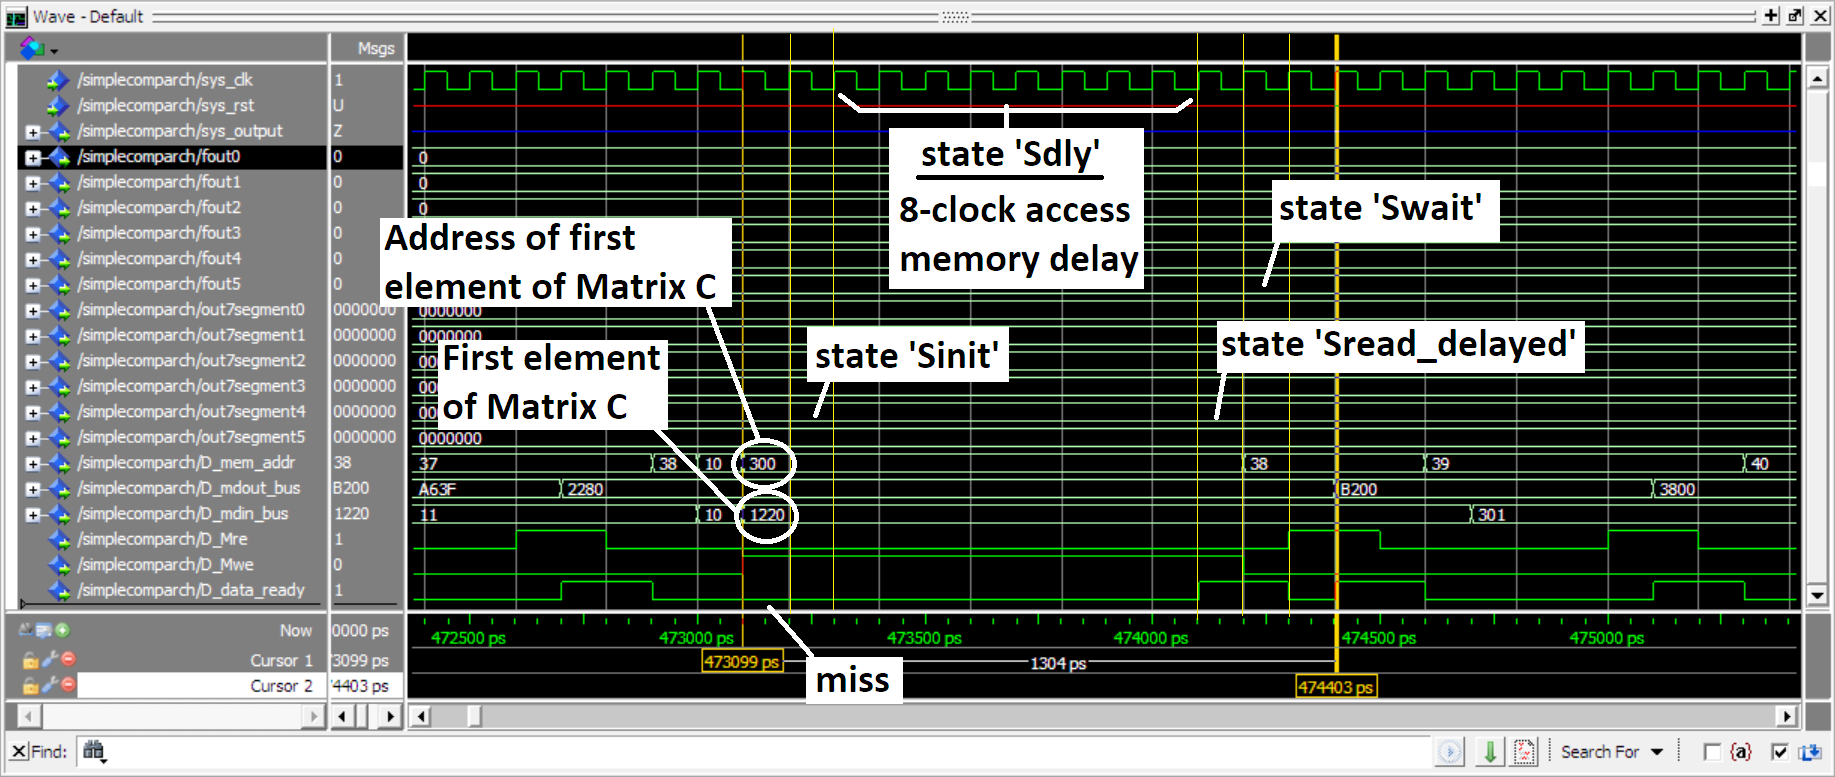
\includegraphics[width=1\linewidth]{./cache/writing_into_cache_memory}}	
	\caption{Cache controller execution.}
	\label{fig:cache2}
\end{figure}

\subsection{Cache memory timing}
Fig. \ref{fig:cache3}b shows that after approx. \textbf{9.41 ns} the multiplication process ends and the first element of resultant Matrix C is displayed, and finally, Fig. \ref{fig:cache3}c displays approx. \textbf{9.93 ns} was used to complete all the \textbf{multiplication and displaying process}.  

\begin{figure}[H]
	\centering
	\subfigure[First element of resultant Matrix C to be displayed in the 7-segment displays.]{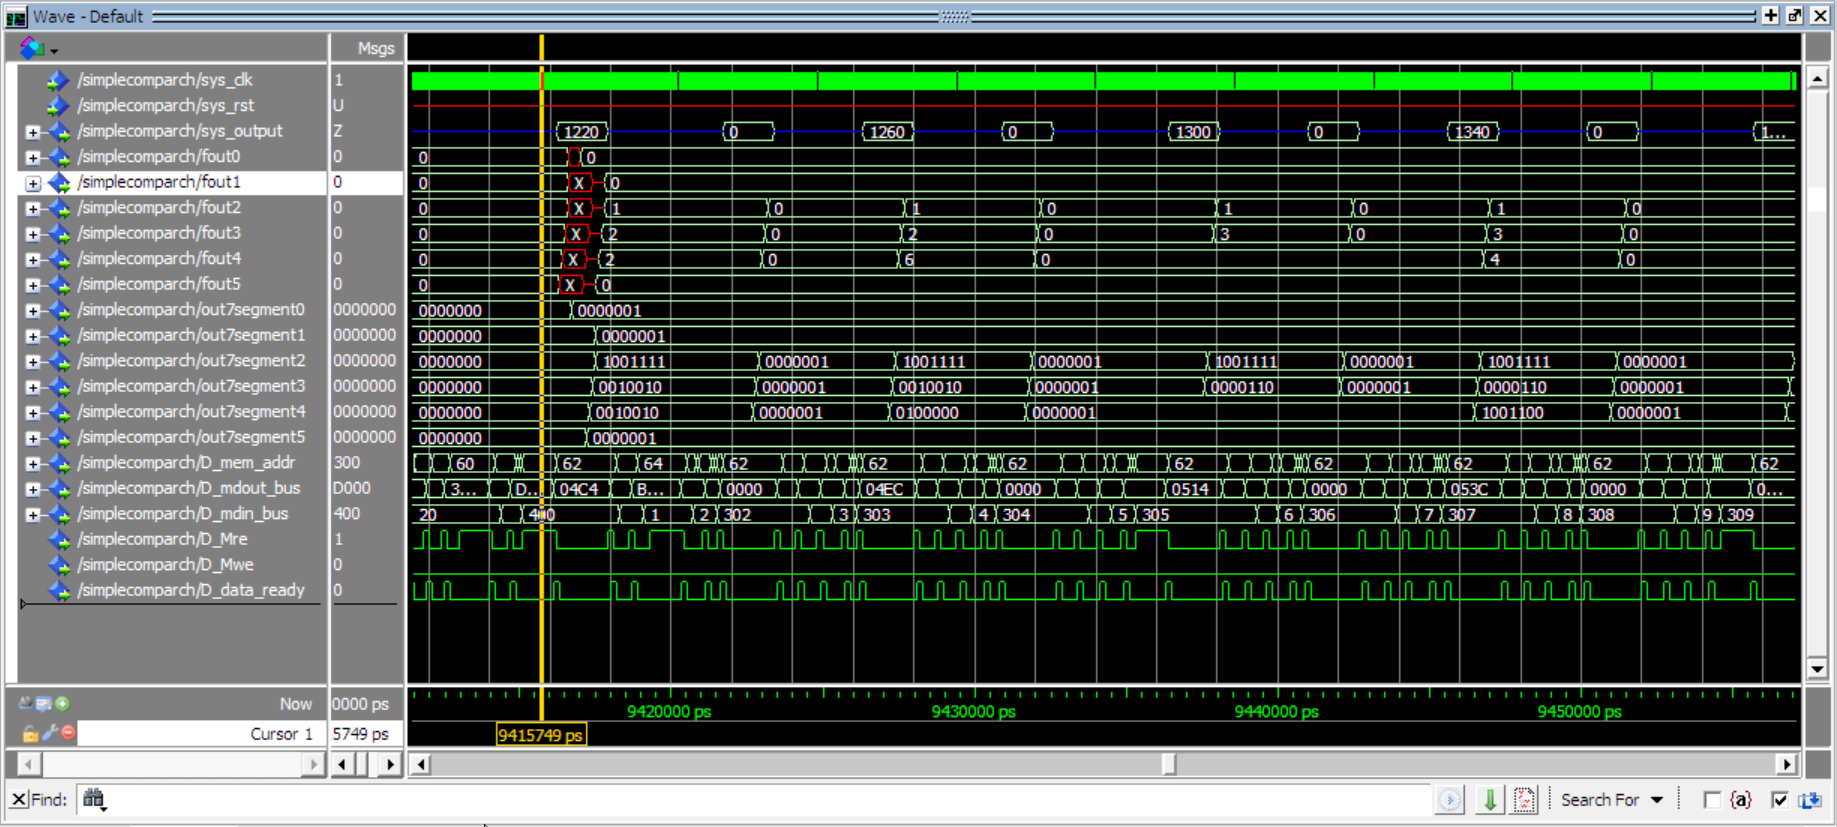
\includegraphics[width=1\linewidth]{./cache/result_start}}
	\subfigure[Last instruction and last displayed element.]{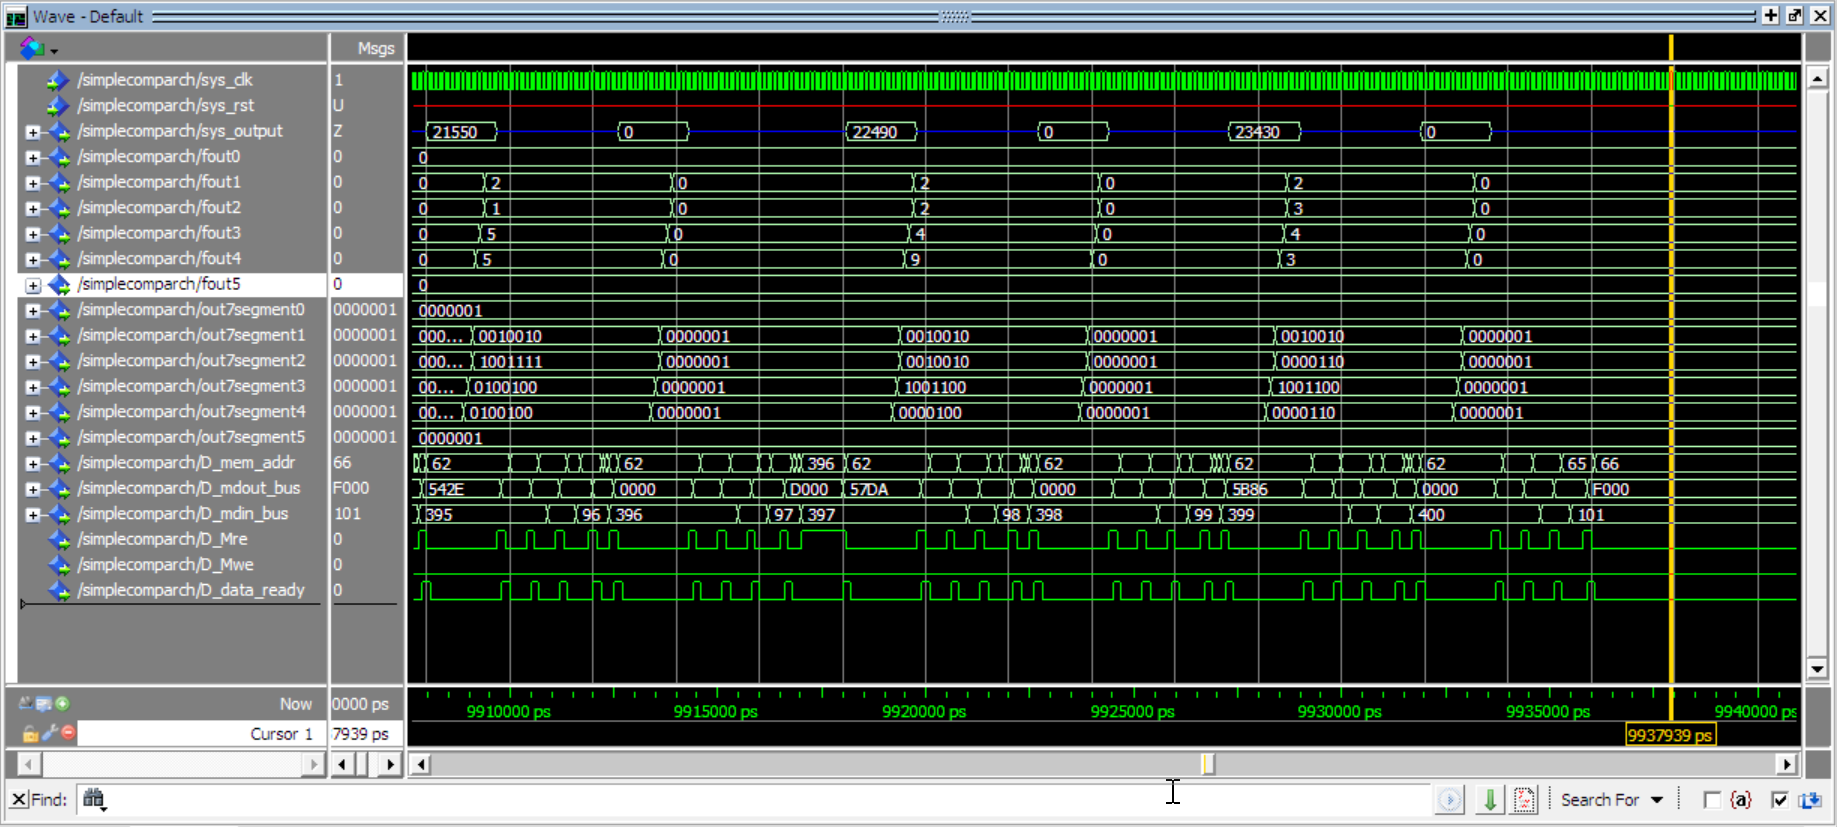
\includegraphics[width=1\linewidth]{./cache/result_end}}		
	\caption{Cache memory simulation.}
	\label{fig:cache3}
\end{figure}

\subsection{Simple memory timing}
Fig. \ref{fig:cache4}b shows that after approx. \textbf{16.36 ns} the multiplication process ends and the first element of resultant Matrix C is displayed, and finally, Fig. \ref{fig:cache4}c displays approx. \textbf{17.22 ns} was used to complete all the \textbf{multiplication and displaying process}.  

\begin{figure}[H]
	\centering
	\subfigure[First element of resultant Matrix C to be displayed in the 7-segment displays.]{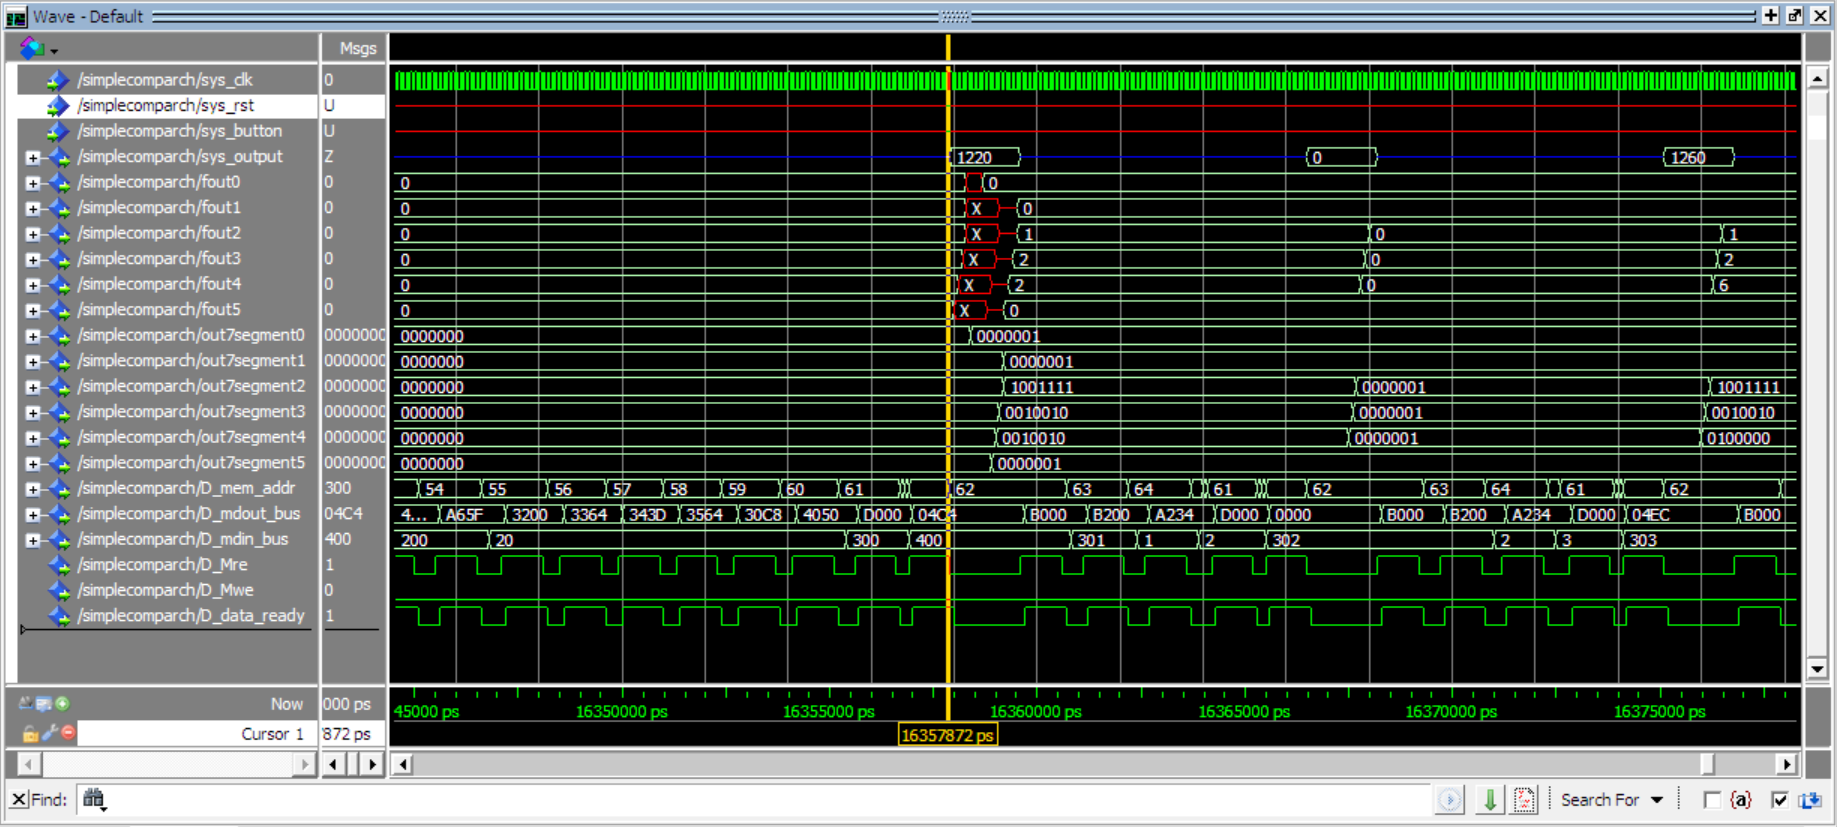
\includegraphics[width=1\linewidth]{./simple_memory/result_start}}
	\subfigure[Last instruction and last displayed element.]{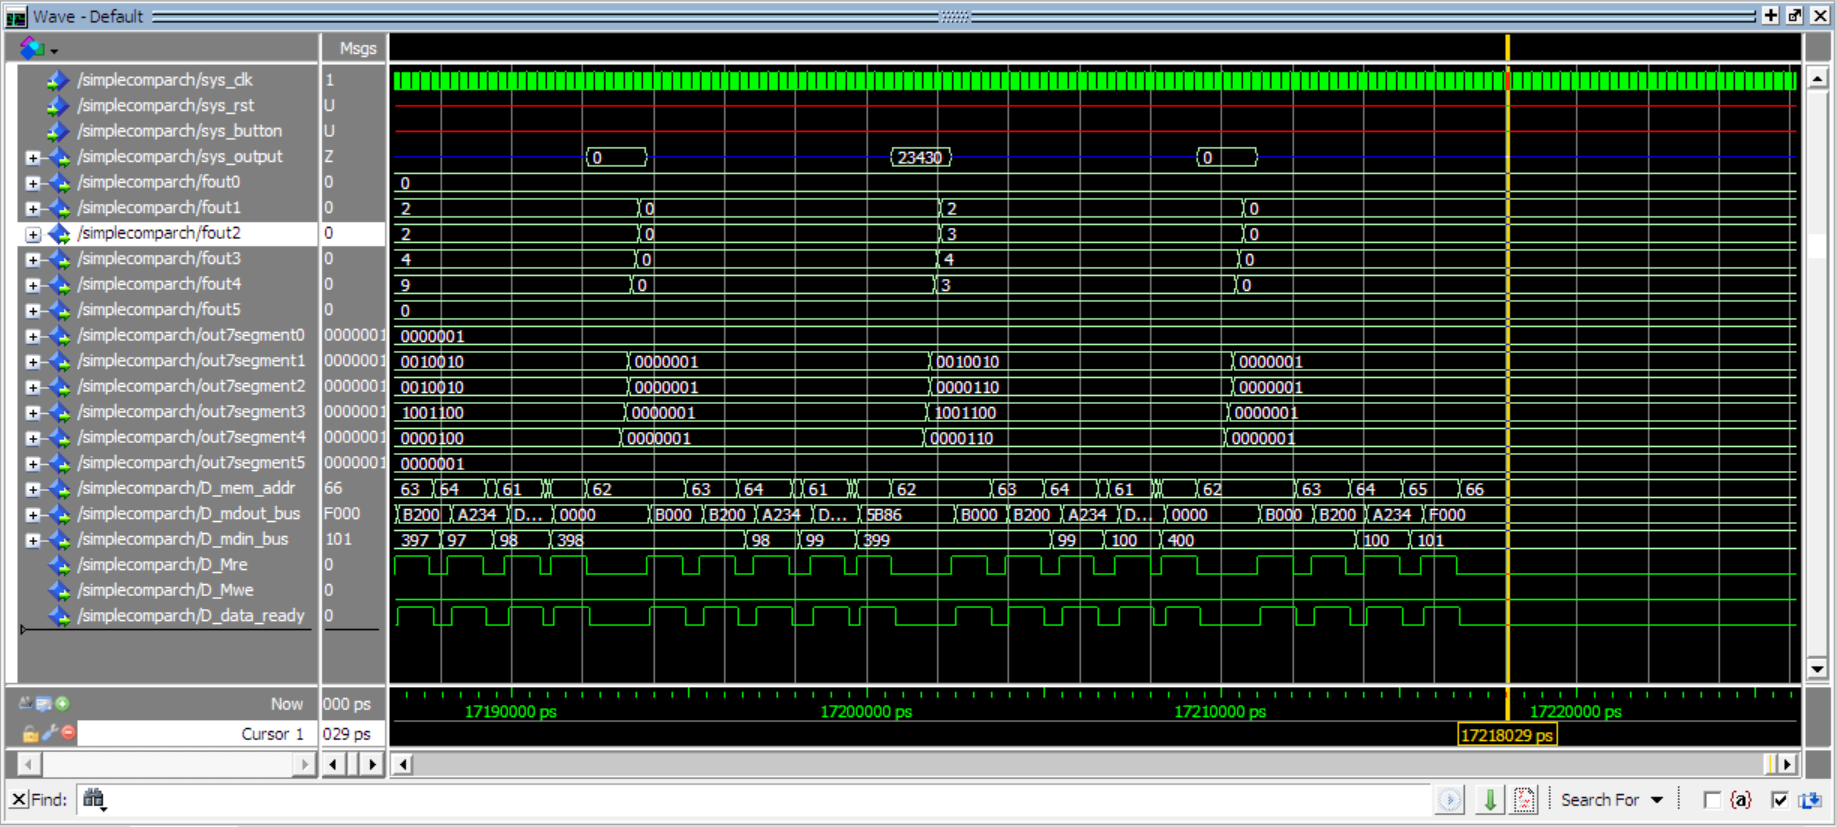
\includegraphics[width=1\linewidth]{./simple_memory/result_end}}		
	\caption{Simple memory simulation.}
	\label{fig:cache4}
\end{figure}

\subsection{Unexpected compilation error}\label{error}
During the compilation process an unexpected error occurred, \verb|Quartus| displayed an over-sized \verb|Logic utilization (in ALMs)| of 191\% that didn't allow us to fit the project into the \verb|DE0-CV| board, Fig. \ref{fig:error}a, so, fitting \verb|Logic utilization| at 92\% we reduce the 12-bit address to 11 bits by reducing the \verb|tag size| from 7 bits to 6 bits.

\begin{figure}[H]
	\centering
	\subfigure[12-bit address compilation.]{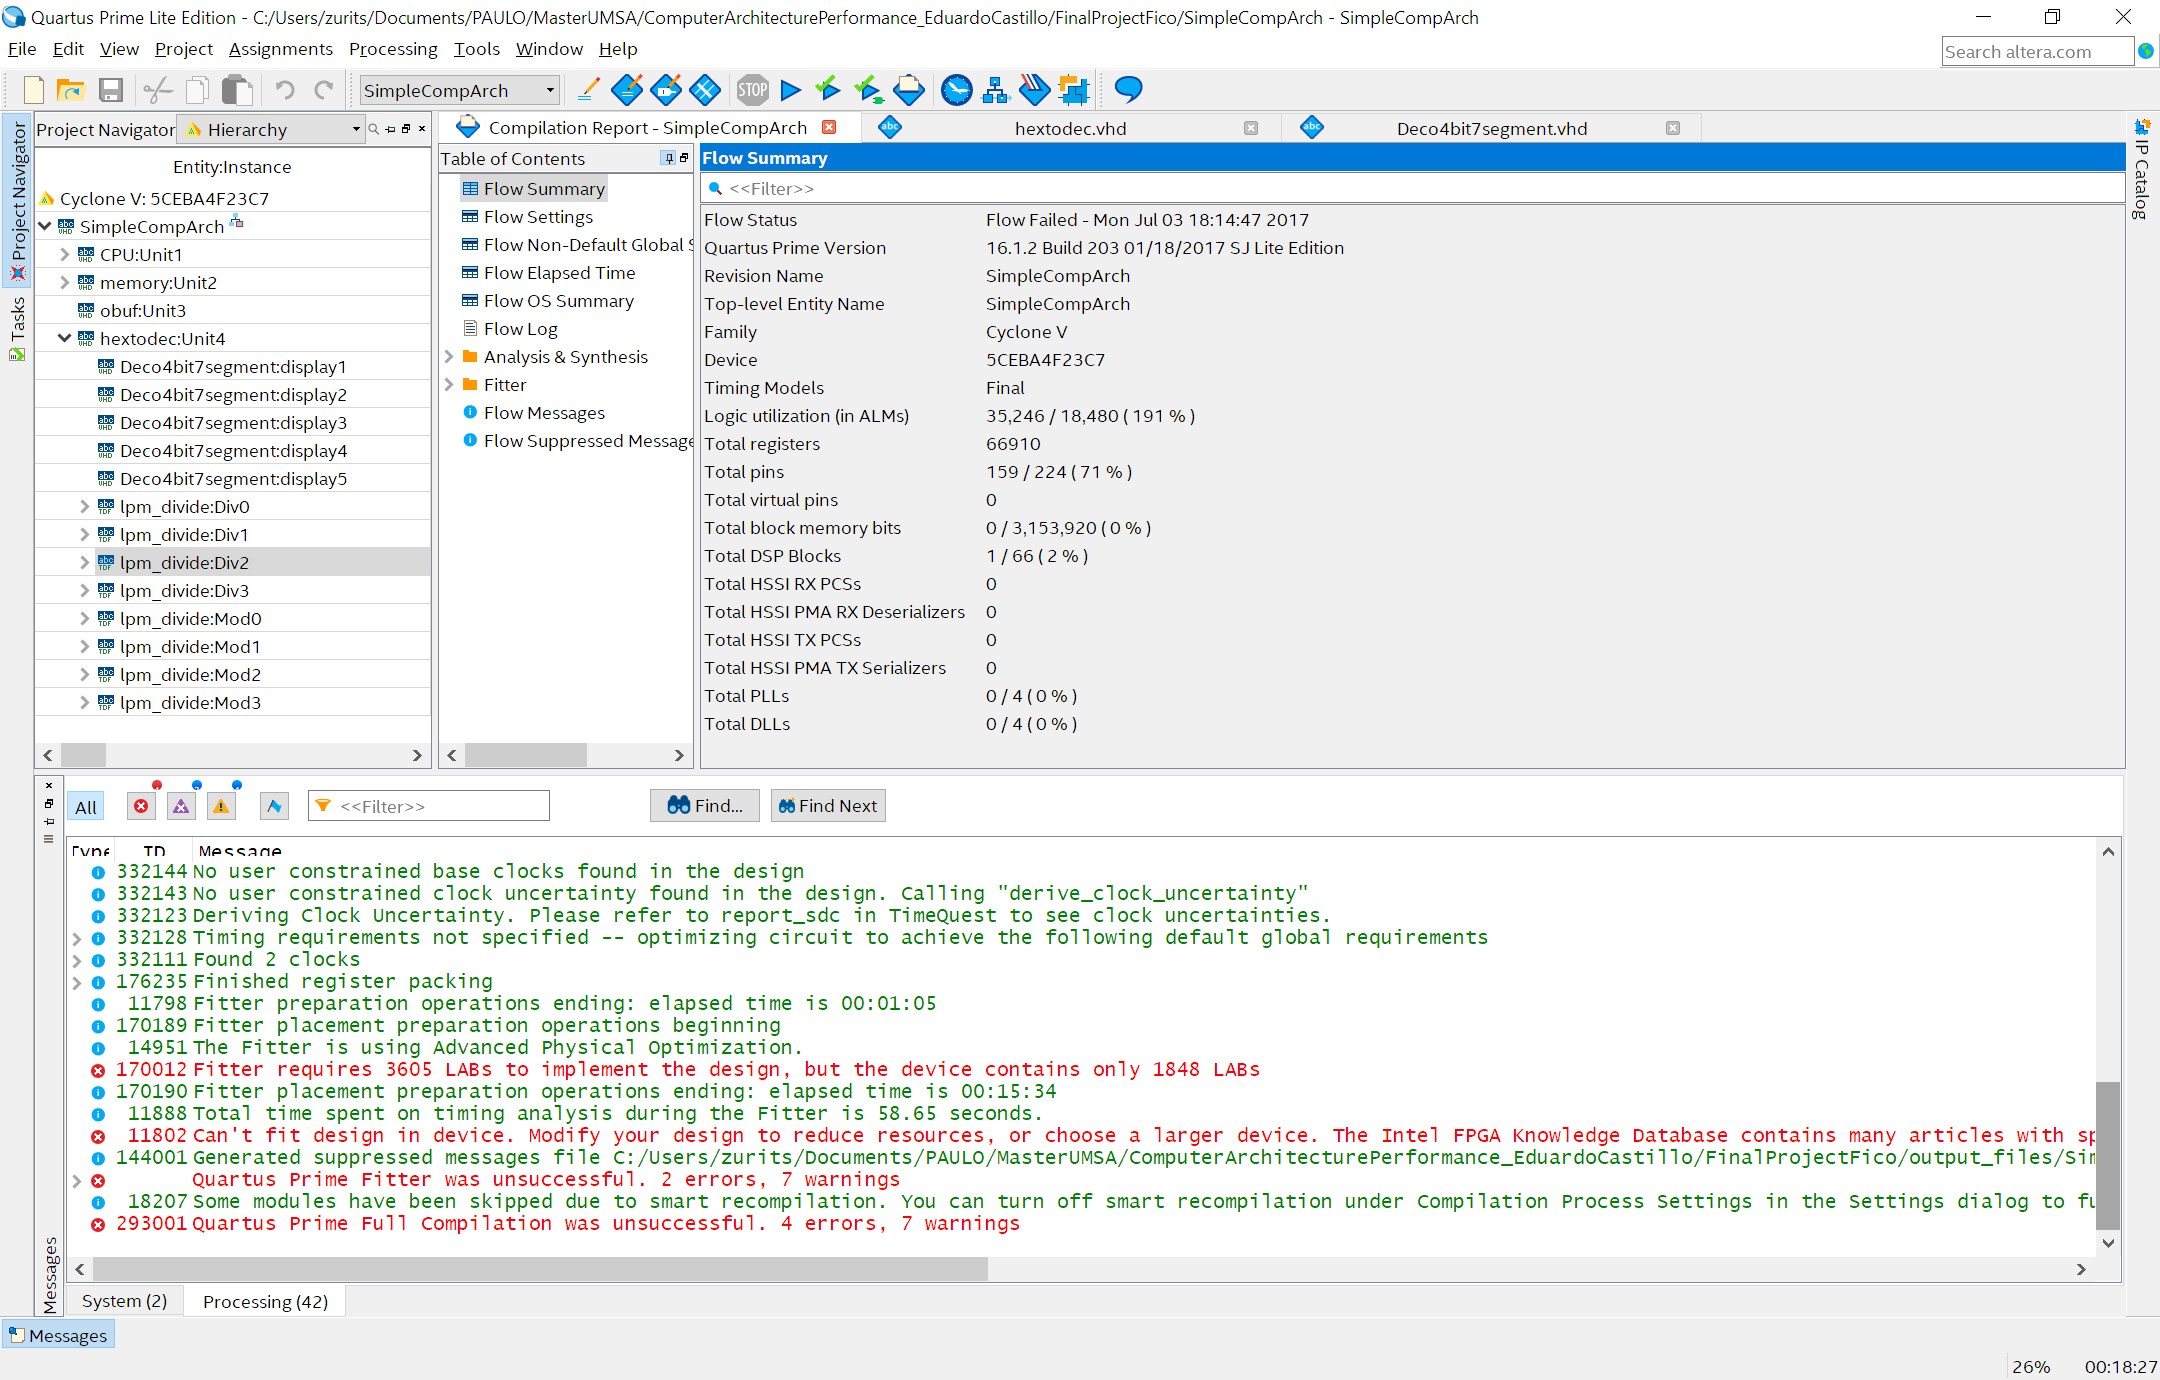
\includegraphics[width=0.7\linewidth]{12bits_address}}
	\subfigure[11-bit address compilation.]{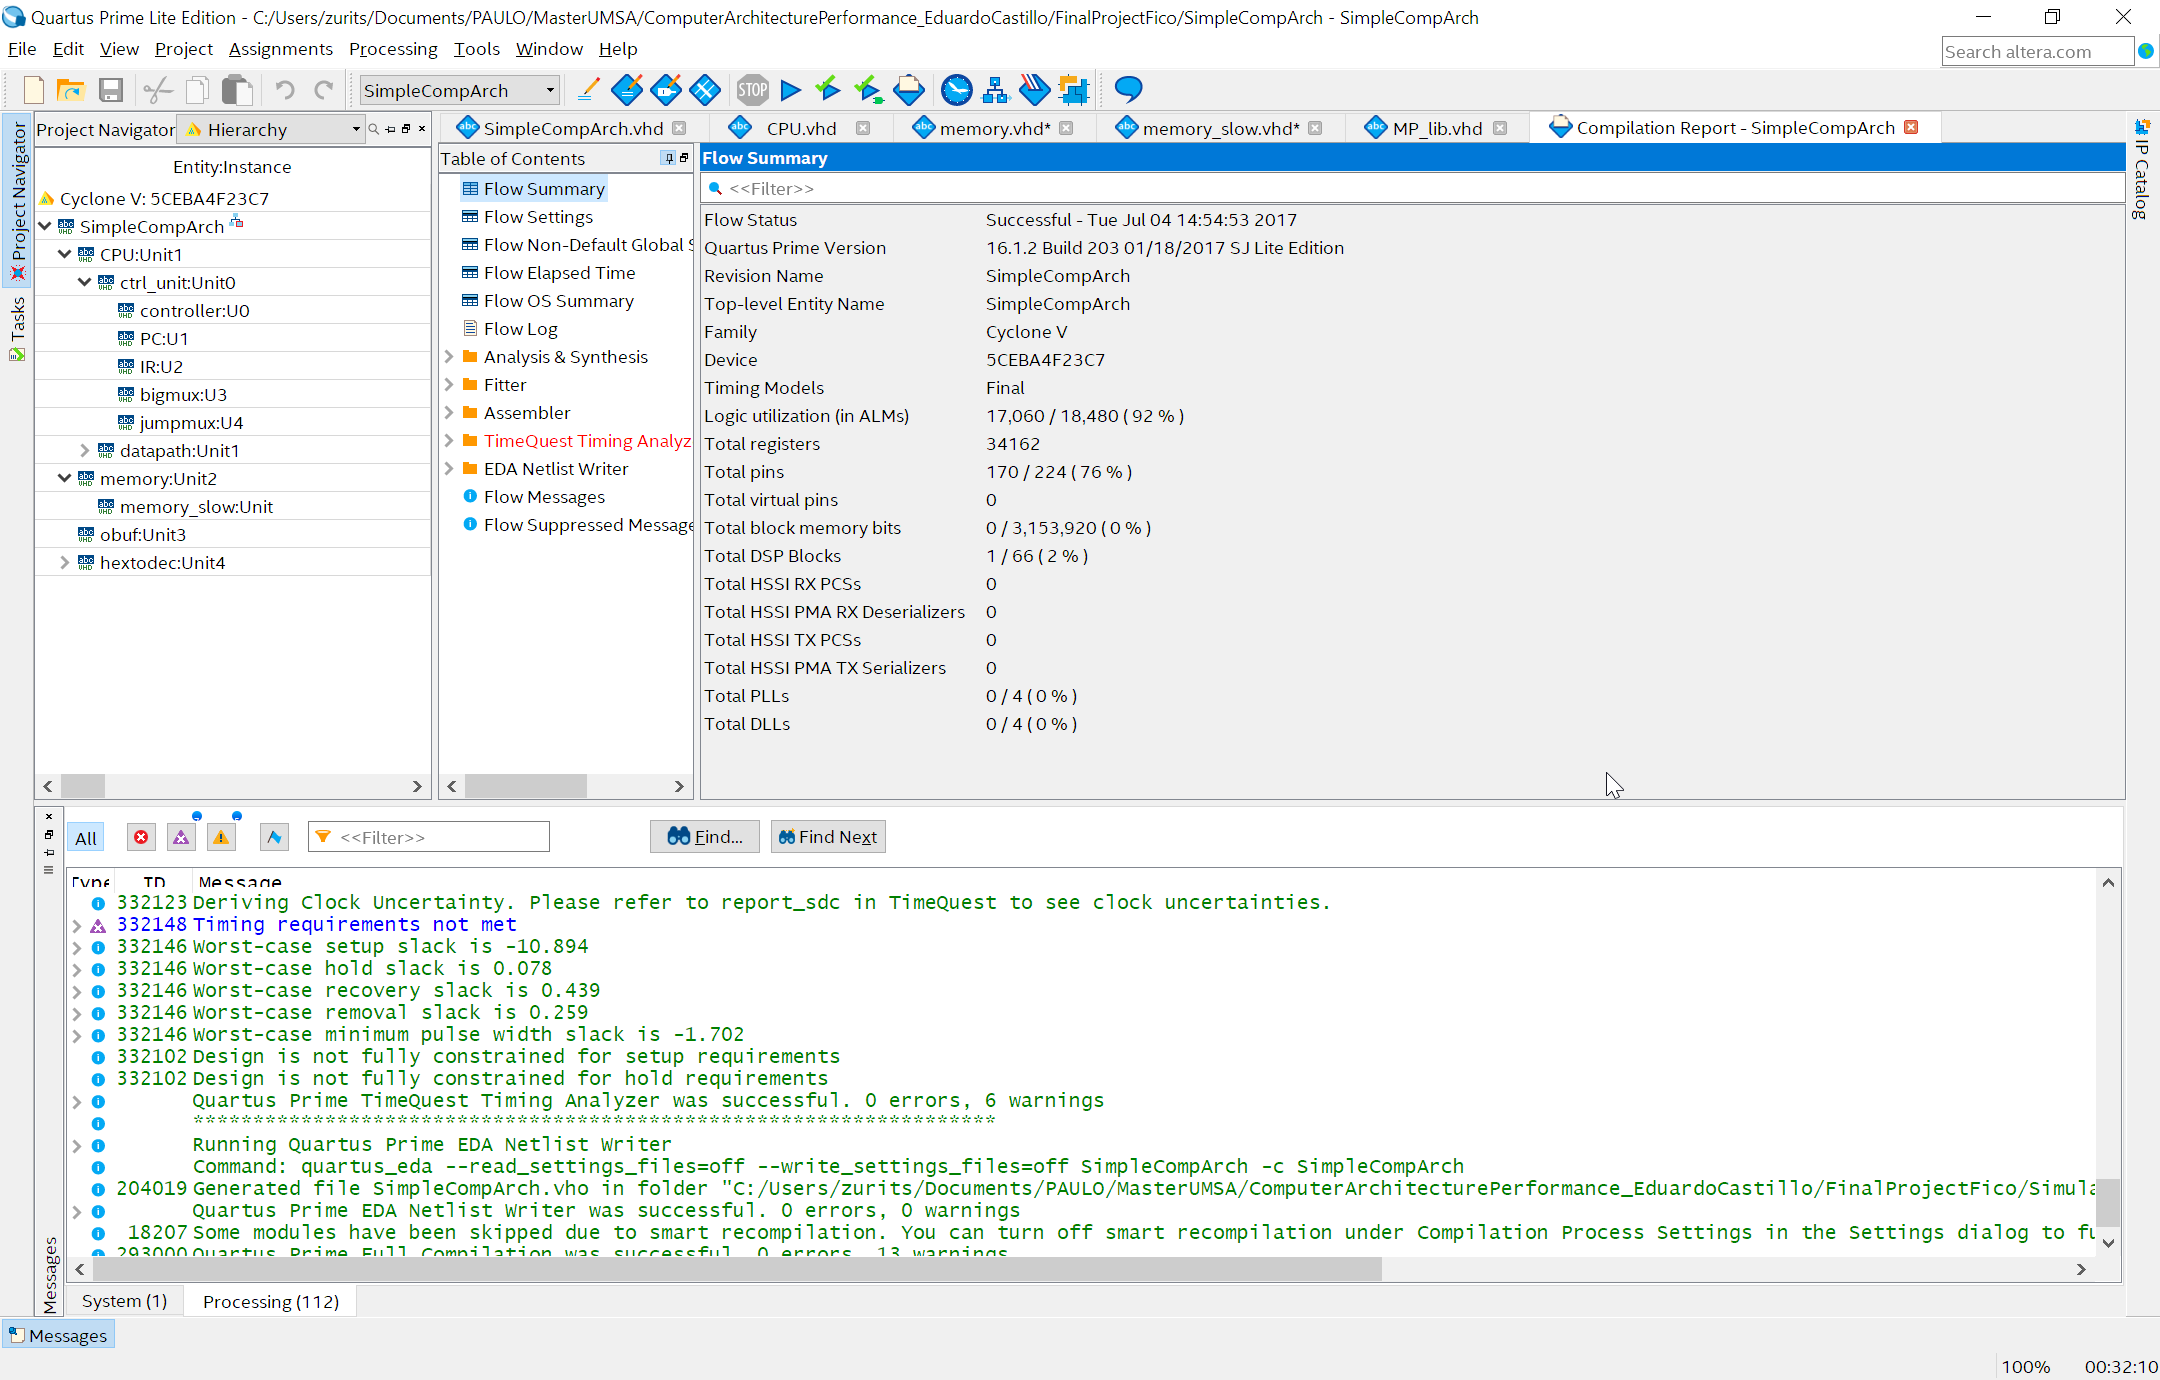
\includegraphics[width=0.7\linewidth]{11bits_address}}		
	\caption{Unexpected compilation error}
	\label{fig:error}
\end{figure}

\section{Conclusions}
The design, simulation and implementation of Direct-mapping cache memory system in VHDL was accomplished and compared it to a reference system without cache memory (simple memory) which is resumed in table \ref{tab:tab1}, that reflects about 50\% of increased performance and can be visualized in Fig. \ref{fig:cache3}b and Fig. \ref{fig:cache4}.
 
\begin{table}[!ht]
	\centering
	\scalebox{1}{
		\begin{tabular}{>{\bfseries}c|c}
			\rowcolor{LightBlue2} \bf{Simple memory (ns)} & \bf{Direct mapped cache memory (ns)} \\ \hline
			                    17.22                     &                 9.93
		\end{tabular} 		
	}
	\caption{Timing simulation results.}
	\label{tab:tab1}
\end{table}

For simulation and implementation purpose, section \ref{comp} established the parameters to compile correctly in order to visualize the results for \verb|ModelSim| and for the \verb|DE0-CV| board.

Finally, a video was edited to visualize the 100 elements of the resultant Matrix C where you can find attached to this .pdf or in the following link \url{https://youtu.be/Zvd96RGTEjk}.

\end{document}
